%% RiSE Latex Template - version 0.5
%%
%% RiSE's latex template for thesis and dissertations
%% http://risetemplate.sourceforge.net
%%
%% (c) 2012 Yguaratã Cerqueira Cavalcanti (yguarata@gmail.com)
%%          Vinicius Cardoso Garcia (vcg@cin.ufpe.br)
%%
%% This document was initially based on UFPEThesis template, from Paulo Gustavo
%% S. Fonseca.
%%
%% ACKNOWLEDGEMENTS
%%
%% We would like to thanks the RiSE's researchers community, the 
%% students from Federal University of Pernambuco, and other users that have
%% been contributing to this projects with comments and patches.
%%
%% GENERAL INSTRUCTIONS
%%
%% We strongly recommend you to compile your documents using pdflatex command.
%% It is also recommend use the texlipse plugin for Eclipse to edit your documents.
%%
%% Options for \documentclass command:
%%         * Idiom
%%           pt   - Portguese (default)
%%           en   - English
%%
%%         * Text type
%%           bsc  - B.Sc. Thesis
%%           msc  - M.Sc. Thesis (default)
%%           qual - PHD qualification (not tested yet)
%%           prop - PHD proposal (not tested yet)
%%           phd  - PHD thesis
%%
%%         * Media
%%           scr  - to eletronic version (PDF) / see the users guide
%%
%%         * Pagination
%%           oneside - unique face press
%%           twoside - two faces press
%%
%%		   * Line spacing
%%           singlespacing  - the same as using \linespread{1}
%%           onehalfspacing - the same as using \linespread{1.3}
%%           doublespacing  - the same as using \linespread{1.6}
%%
%% Reference commands. Use the following commands to make references in your
%% text:
%%          \figref  -- for Figure reference
%%          \tabref  -- for Table reference
%%          \eqnref  -- for equation reference
%%          \chapref -- for chapter reference
%%          \secref  -- for section reference
%%          \appref  -- for appendix reference
%%          \axiref  -- for axiom reference
%%          \conjref -- for conjecture reference
%%          \defref  -- for definition reference
%%          \lemref  -- for lemma reference
%%          \theoref -- for theorem reference
%%          \corref  -- for corollary reference
%%          \propref -- for proprosition reference
%%          \pgref   -- for page reference
%%
%%          Example: See \chapref{chap:introduction}. It will produce 
%%                   'See Chapter 1', in case of English language.
%%
%% Citation commands:
%%          \citet (from natbib) -- To cite a reference as part of the narrative
%%          \citep (from natbib) -- To cite a reference between parenthesis
%%          citationblock environment -- To produce direct citation blocks according to the ABNT

\documentclass[pt,oneside,onehalfspacing,bsc]{risethesis}
%antes tinha twoside

%\usepackage{hyperref}
\usepackage{colortbl}
\usepackage{color}
\usepackage[table]{xcolor}
\usepackage{xwatermark} 
\usepackage{microtype}
\usepackage{bibentry}
\usepackage{subfigure}
\usepackage{multirow}
\usepackage{rotating}
\usepackage{booktabs}
\usepackage{pdfpages}
\usepackage{caption}
\usepackage{lipsum}
\usepackage{sectsty}
\usepackage{graphicx}
\usepackage{transparent}
\usepackage{eso-pic}
\usepackage{pdfpages}
\usepackage{float}
%\usepackage{abntcite}

\captionsetup[table]{position=top,justification=centering,width=.85\textwidth,labelfont=bf,font=footnotesize}
\captionsetup[lstlisting]{position=top,justification=centering,width=.85\textwidth,labelfont=bf,font=footnotesize}
\captionsetup[figure]{position=bottom,justification=centering,width=.85\textwidth,labelfont=bf,font=footnotesize}

%% Chapter and (Sub)Section fonts must be same size as text (12)
\sectionfont{\fontsize{12}{15}\selectfont}
\subsectionfont{\fontsize{12}{15}\selectfont}
\subsubsectionfont{\fontsize{12}{15}\selectfont}

%% Change the following pdf author attribute name to your name.
\usepackage[linkcolor=black,
            citecolor=black,
            urlcolor=black,
            colorlinks,
            pdfpagelabels,
            pdftitle={Rise Thesis Template (ABNT)},
            pdfauthor={Rise Thesis Template (ABNT)},
            breaklinks=true]{hyperref}
%\usepackage{abntex2cite}

\address{RECIFE}

\universitypt{Universidade Federal de Pernambuco}
\universityen{Federal University of Pernambuco}

\departmentpt{Centro de Informática}
\departmenten{Center for Informatics}

\programpt{Graduação em Engenharia da Computação}
\programen{Graduate in Computer Engineering}

\majorfieldpt{Engenharia da Computação}
\majorfielden{Computer Engineering}

\title{Um Estudo Sobre Propriedade Intelectual em Hackathons}

\date{2020}

\author{Geraldo Pereira da Silva Júnior}
\adviser{Kiev Santos da Gama}

% Macros (defines your own macros here, if needed)
\def\x{\checkmark}

\begin{document}

\frontmatter

\frontpage

\AddToShipoutPicture{
\put(0,0){
\parbox[b][\paperheight]{\paperwidth}{%
\vfill
\centering
{\transparent{0.4}
\includegraphics[width=1.1\textwidth]{images/ufpedagua.png}}
\vfill}}}

\presentationpage

\begin{fichacatalografica}
	\FakeFichaCatalografica % Comment this line when you have the correct file
%     \includepdf{fig_ficha_catalografica.pdf} % Uncomment this
\end{fichacatalografica}

\banca

\begin{dedicatory}
Eu dedico este trabalho a toda minha família, amigos e professores que foram fundamentais e me deram o suporte necessário para chegar até aqui.%
%I dedicate this thesis to all my family, friends and professors who gave me the necessary support to get here.
\end{dedicatory}

\acknowledgements
Primeiramente agradecer a Deus por me proporcionar perseverança, fé e me ajudar nas realizações mais complicadas durante toda a minha vida.

Aos meus pais Geraldo e Cristina pelo apoio e incentivo que serviram de alicerce para as minhas conquistas. A minha irmã Graziela pela amizade e atenção dedicadas quando sempre precisei.

Ao meu professor orientador Kiev pelas valiosas contribuições e orientações dadas durante todo o processo.

Aos meus amigos da vida, da igreja e do clube de Desbravadores que ao longo da jornada me ensinou a ser uma pessoa melhor.

A todos os meus amigos do curso de graduação que compartilharam dos inúmeros desafios que enfrentamos, as diversas noites madrugadas para realizar os projetos e listas de exercício, sempre com o espírito colaborativo.

Também quero agradecer à Universidade Federal de Pernambuco e o seu corpo docente que demonstrou estar comprometido com a qualidade e excelência do ensino.

\begin{epigraph}[]{Stephen Fry}
"An original idea. That can't be too hard. The library must be full of them."
\end{epigraph}

\resumo
\ClearShipoutPicture
% Escreva seu resumo no arquivo resumo.tex
{\parindent0pt
	Entusiasmo, empolgação, regalias, são alguns dos fatores que levam uma pessoa a participar de hackathons, eventos baseados em duração temporal onde os participantes buscam superar-se e superar seus adversários e colegas através de desafios que geralmente duram um final de semana carregados de brindes e diversão. Mas será que todos os participantes estão atentos aos regulamentos e até onde eles têm prioridade em seus direitos? Através deste estudo buscamos entender a percepção dos competidores das hackathons a fim de compreender melhor o entendimento e compreensão sobre os seus direitos à propriedade intelectual em determinada hackathon. Através de entrevistas semi-estruturadas e uma \textit{survey} para melhor compreender as percepções e entendimentos dos participantes. Como resultado ainda existe um relaxamento quanto a clareza e melhores definições nos regulamentos, assim levando o participante a não compreender a cessão ou não cessão dos direitos à PI em uma determinada hackathon.  


\begin{keywords}
Hackathon, Propriedade Intelectual, Crowdsourcing, Time-Bounded Events, Percepção
\end{keywords}
}

\abstract
% Write your abstract in a file called abstract.tex
{\parindent0pt
	Enthusiasm, excitement, perks, are some of the factors that lead a person to participate in hackathons, time-bounded events where participants seek to overcome themselves and overcome their opponents and colleagues through challenges that usually last a weekend laden with gifts and fun. But are all participants aware of the regulations and how far do they have priority over their rights? Through this study we seek to understand the perception of hackathons' competitors in order to better understand the knowledge and comprehension of their intellectual property rights in a given hackathon. Through semi-structured interviews and a survey to better understand the participants' perceptions and comprehension. As a result, there is still a relaxation in terms of clarity and better definitions in the regulations, thus leading the participant to not understand the assignment or non-assignment of rights to IP in a given hackathon.

\begin{keywords}
Intelectual Property, Hackathon, Time-bounded Events, Crowdsourcing, Perception
\end{keywords}
}

% List of figures
\listoffigures

% List of tables
\listoftables

% List of acronyms
% Acronyms manual: http://linorg.usp.br/CTAN/macros/latex/contrib/acronym/acronym.pdf
\listofacronyms
\begin{acronym}[ACRONYM] 
% Change the word ACRONYM above to change the acronym column width.
% The column width is equals to the width of the word that you put.
% Read the manual about acronym package for more examples:
%   http://linorg.usp.br/CTAN/macros/latex/contrib/acronym/acronym.pdf
\acro{afm}[AFM]{Alphabet Frequency Matrix}
\acro{api}[API]{Application Programming Interface}
\acro{arima}[ARIMA]{Auto-Regressive Integrated Moving Average}
\acro{brn}[BRN]{Bug Report Network}
\acro{bts}[BTS]{Bug Triage System}
\acro{cas}[CAS]{Context-Aware Systems}
\acro{ccb}[CCB]{Change Control Board}
\acro{cr}[CR]{Change Request}
\acro{cvs}[CVS]{Concurrent Version System}
\acro{es}[ES]{Expert System}
\acro{floss}[FLOSS]{Free/Libre Open Source Software}
\acro{glr}[GLR]{Generalized Linear Regression}
\acro{gqm}[GQM]{Goal Question Metric}
\acro{html}[HTML]{HyperText Markup Language}
\acro{ir}[IR]{Information Retrieval}
\acro{irt}[IRT]{Recôncavo Institute of Technology}
\acro{jdt}[JDT]{Jazz Duplicate Finder}
\acro{lda}[LDA]{Latent Dirichlet Allocation}
\acro{loc}[LOC]{Lines of Code}
\acro{lsi}[LSI]{Latent Semantic Indexing}
\acro{ms}[MS]{Mapping Study}
\acro{msr}[MSR]{Mining Software Repositories}
\acro{nlp}[NLP]{Natural Language Processing}
\acro{promise}[PROMISE]{Predictive Models in Software Engineering}
\acro{rbes}[RBES]{Rule-Based Expert System}
\acro{rhel}[RHEL]{RedHat Enterprise Linux}
\acro{saas}[SaaS]{Software as a Service}
\acro{scm}[SCM]{Software Configuration Management}
\acro{serpro}[SERPRO]{Brazilian Federal Organization for Data Processing}
\acro{slr}[SLR]{Stepwise Linear Regression}
\acro{slr}[SLR]{Systematic Literature Review}
\acro{svd}[SVD]{Singular Value Decomposition}
\acro{svm}[SVM]{Support Vector Machine}
\acro{svn}[SVN]{Subversion}
\acro{tfidf}[TF-IDF]{Term Frequency-Inverse Document Frequency}
\acro{vsm}[VSM]{Vector Space Model}
\acro{xp}[XP]{Extreming Programming}
%%%%%%%%%%%%%%%%%%%%%%%%%%%%%%%%% DOS MEUS %%%%%%%%%%%%%%%%%%%
\acro{pi}[PI]{Propriedade Intelectual}
\acro{inpi}[INPI]{Instituto Nacional da Propriedade Industrial}
\acro{ompi}[OMPI]{Organização Mundial de Propriedade Intelectual}
\acro{wipo}[WIPO]{World Intelectual Property Organization}
\end{acronym}

% Summary (tables of contents)
\tableofcontents

\mainmatter
%%%%% CAPITULOS %%%% 
\chapter{Introdução}
\label{chp:introdução}

Eventos de programação voltados a criar soluções inovadoras para um determinado problema específico estão na moda. A busca por soluções otimizadas e cada vez mais econômicas motiva os  organizadores a idealizarem desafios cada vez mais inovadores nas hackathons.


Em termos leigos pode-se dizer que hackathons são eventos de maratonas hackers de exploração de novas ideias e produtos, em sua maioria voltados para tecnologia e/ou questões sociais. \citep{briscoe2014digital}

Desenvolvedores de software, designers e outros profissionais relacionados à área de programação participam desses eventos que trazem diversos benefícios às empresas, quer sejam \textit{startups} ou empresas tradicionais em busca de inovação. Auxiliando-as no desenvolvimento de novas tecnologias e apresentando novos talentos.

\citet{zukin2017hackathons} cita diversos pontos em que os participantes, em meio a empolgação do evento, negligenciam, ou lembram de forma mínima. Um deles é o tópico sobre com quem fica a PI do código produzido no evento, onde em alguns casos é dúbia a definição. \citep{steele_2013}

\citet{zukin2017hackathons} também afirma que em meio a tanta inovação, recreação e oportunidades de crescer o portfólio individual de cada participante, existe um lado negro muito forte, onde os participantes lutam por premiações abaixo do valor necessário, passam dias confinados em ambientes insalubres. É visto como estratégia para empresários da tecnologia explorarem os participantes em busca de soluções baratas e rápidas.


Para melhorar o entendimento dos participantes foi criado o \textit{The Hack Day Manifesto}\footnote{The Hack Day Manifesto <https://hackdaymanifesto.com/>}, onde informa sobre alguns requerimentos básicos que ajudam no sucesso da Hackathon. Um guia completo e sugestivo, com detalhes, para evitar dualidades de entendimento no evento e em seu regulamento.

No Brasil, no ano de 2016, ocorreu uma hackathon promovido pela empresa Gerdau. O qual chamou muito a atenção para alguns pontos que foram tratados como "pegadinha" dos organizadores para os participantes mais desavisados. 

Na 10ª cláusula, que trata da propriedade intelectual lê-se no segundo item:
\begin{quote}
    "Os participantes se obrigam a ceder à Gerdau, de forma não onerosa e exclusiva, todos os direitos patrimoniais decorrentes dos projetos desenvolvidos durante o Evento, sempre reservando para si os direitos morais a eles associados. Os participantes ainda declaram ser livres de quaisquer ônus ou embaraços à Gerdau os direitos patrimoniais ora cedidos."\footnote{Regulamento retirado do ar, mas pode ser encontrado em: <https://docplayer.com.br/23433151-Regulamento-hackathon-gerdau-2016.html>. Acessado em 20 de mar. 2020}
\end{quote} 
Onde todos os direitos sobre as ideias desenvolvidas são de propriedade da Gerdau e não dos desenvolvedores.

Por fim, o quarto item diz:
\begin{quote}
    "Os participantes serão responsáveis pela utilização de suas ideias e pela elaboração de seu projeto, assumindo total e exclusiva responsabilidade decorrente de eventuais reivindicações de terceiros relativos a direitos de propriedade intelectual ou de direito autoral, sendo preservado o direito de regresso ou de denunciação à lide em razão de eventuais questionamentos de terceiros."\footnote{Regulamento retirado do ar, mas pode ser encontrado em: <https://docplayer.com.br/23433151-Regulamento-hackathon-gerdau-2016.html>. Acessado em 20 de mar. 2020}
\end{quote}

Os desenvolvedores responsabilizam-se legalmente sobre suas criações. A Gerdau exime-se de quaisquer responsabilidade e problemas posteriores, tais como acusações de plágio, onde os desenvolvedores responderão pelos atos.

A Gerdau, neste caso, utilizou o nome Hackathon para absorver ideias dos participantes sem custo, não iria pagar direitos de propriedade intelectual e nem de imagem, e caso haja algum problema legal, quem responderia seriam os criadores e não a empresa, sem deixar muito claro aos participantes, principalmente os mais desavisados.

Este trabalho tem como objetivo analisar e compreender como a propriedade intelectual é percebida pelos participantes de hackathons e como as empresas expressam em seus regulamentos a quem pertence os direitos de propriedade intelectual. Para isso foram realizadas surveys e entrevistas semi-estruturadas como forma de coleta de dados a respeito dos participantes e análise de regulamentos de hackathons. Diante do objetivo geral serão realizadas pesquisas quantitativas e qualitativas sobre o assunto e serão propostas formas de como melhorar a qualidade e percepção da propriedade intelectual para os competidores.
\chapter{Fundamentação Teórica}
\label{chp:fundamentaçãoTeórica}


\section{Propriedade Intelectual}

De acordo com \citet{WIPO2016} e \citet{howe2013concepts} o conceito de Propriedade Intelectual é definido como uma categoria de propriedade, que inclui criações intangíveis do intelecto humano, seja nos domínios industrial, científico, literário ou artístico. Por meio de leis é garantido aos responsáveis ou inventores quaisquer produção feita por eles.

A \ac{ompi} ou \textit{\ac{wipo}}\footnote{WIPO <https://www.wipo.int/portal/en/index.html> 
} divide a Propriedade Intelectual em três segmentos principais: os  direitos  autorais,  os  de Propriedade  Industrial,  e  outros  direitos  sobre  bens  imateriais  de  vários  gêneros (Proteção \textit{Sui Generis}\footnote{Os tipos de proteção sui generis abrangem desde as cultivares, as topografias de circuito integrado e os conhecimentos tradicionais;}),  conforme  ilustra \autoref{fig:PI}.

\begin{figure}[H]
\centering
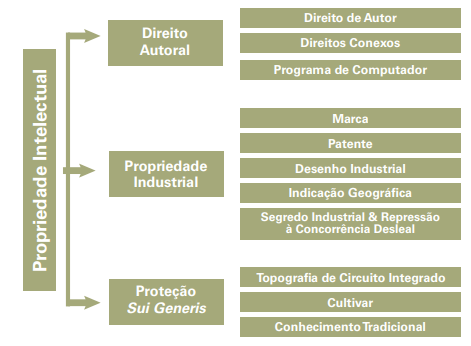
\includegraphics[]{images/modalidades}
\caption{Fonte: \citep{jungman2010}}
\label{fig:PI}
\end{figure}

Segundo \citet{buainain2005propriedade}, a propriedade intelectual:%definição
\begin{quote}
    "Possibilita transformar o conhecimento, em princípio um bem quase público, em bem privado e é o elo de ligação entre o conhecimento e o mercado."
\end{quote}

A razão da existência dos direitos à propriedade intelectual é impedir o uso não autorizado, a venda, fabricação ou importação de um produto similar na esfera de sua proteção de acordo com as leis vigentes. Justamente para que pessoas de má fé não tirem proveito do direito alheio.


\subsection{Lei Brasileira sobre \ac{pi}} 
No Brasil, existe uma lei específica que trata do assunto de propriedade intelectual, onde se dispõe sobre a proteção da propriedade intelectual de programa de computador, sua comercialização no país, além de mostrar providências relacionadas ao assunto. 

A proteção  é a mesma dada às obras literárias pela lei que trata dos direitos autorais. Além dessa lei, há uma legislação específica que trata do assunto: a Lei nº 9.609, de 19 de fevereiro de 1998, conhecida como Lei do Software\footnote{Disponível em: <http://www.planalto.gov.br/civil\_03/leis/L9609> Acesso em 17 mar. 2020}. %precisa referenciar no final?

O site do Instituto Nacional da Propriedade Industrial, afirmando o Decreto de Berna \citep{leideBerna} diz que: 

\begin{quote}
    "O registro de programa de computador é válido por 50 anos a partir da sua criação ou de 1º de janeiro do ano subsequente à sua publicação. A proteção não é territorial, isto é, sua abrangência é internacional, compreendendo os 175 países signatários da Convenção de Berna (1886)." \footnote{Fonte: <http://www.inpi.gov.br/servicos/perguntas-frequentes-paginas-internas/perguntas-frequentes-programa-de-computador>. Acessado em: 19 mar. 2020} \citep{leideBerna}
\end{quote}


A Lei de Direito Autoral (Lei nº 9.610/1998)\footnote{Fonte: <http://www.planalto.gov.br/ccivil\_03/leis/L9610.htm>. Acessado em: 19 mar. 2020}", juntamente com a Lei de Software (Lei nº 9.609/1998)", garantem proteção ao programa de computador em si, à expressão literal do software, isto é, suas linhas de código-fonte. Ao registrar o programa de computador no IMPI, obtém-se as garantias jurídicas necessárias para proteger o autor daquele código-fonte, inclusive, por exemplo, em situações de uma demanda judicial para comprovar a autoria ou titularidade do programa.

Não existe limitações com relação à quantidade de registros sobre um mesmo software e suas diferentes versões. Assim é possível garantir a máxima extensão para a proteção ao código-fonte. \citep{inpiPerguntasFrequentes} 

\begin{quote}
    "Aqui vale uma ressalva: softwares apenas conceituais, ou seja, programas de computador que ainda se encontrem meramente no campo da ideia, não são passíveis de proteção." \citep{inpiPerguntasFrequentes}
\end{quote}

Portanto implementações conceituais, precisam estar documentadas e implementadas, mesmo que de forma incompleta, para que seja validados os seus registros. 

Quanto o desenvolvimento do software está associado a uma relação de trabalho ou prestação de serviço, a indicação na lei é que os direitos relativos ao programa pertencem ao empregador, contratante ou órgão público, salvo quando há uma disposição contrária, quando o acordo contratual define. \citep{lei9609/98}

Assim de acordo com o artigo 28 da Lei 9.610/98 
\begin{quote}
    cabe ao Autor, ou ao detentor dos direitos autorais patrimoniais o direito exclusivo de utilizar, fruir e dispor da obra literária, artística ou científica”; \citep{lei9610/98}
\end{quote}“ 
e o artigo 29 da mesma lei
\begin{quote}
    “depende de autorização prévia e expressa do mesmo para que a obra seja utilizada, por quaisquer modalidades, dentre elas a reprodução parcial ou integral”. \citep{lei9610/98}
\end{quote}
Toda cópia reproduzida de forma não autorizada constitui de um ato ilícito civil e criminal, passível de punição de acordo com a lei brasileira.

\subsection{Licenças de Código Aberto  e Software Livre}

Existem iniciativa importantes que visam flexibilizar restrições e proteções relativas aos direitos autorais, são conhecidas como iniciativas de Código Aberto (do inglês \textit{"Open Source"} e o Software Livre. São iniciativas distintas que baseiam em conceder aos usuários liberdade para executar, copiar, distribuir e modificar o software, sem que haja transgressão aos direitos autorais.


De acordo com o site da GNU, software livre é definido como o respeito à liberdade e o senso de comunidade existente entre os usuários, dando liberdade para executar, copiar, distribuir, estudar e/ou melhorar o software. Algo que deve ser ressaltado é o fato do software livre não ser confundido com software grátis, são conceitos diferentes, onde alguns softwares livres podem ser gratuitos. \citep{gnu}

\begin{quote}
"Um programa é software livre se os usuários possuem as quatro liberdades essenciais:
\begin{itemize}
    \item liberdade de executar o programa como você desejar, para qualquer propósito (liberdade 0).
    \item liberdade de estudar como o programa funciona, e adaptá-lo às suas necessidades (liberdade 1). Para tanto, acesso ao código-fonte é um pré-requisito.
    \item liberdade de redistribuir cópias de modo que você possa ajudar outros (liberdade 2).
    \item liberdade de distribuir cópias de suas versões modificadas a outros (liberdade 3). Desta forma, você pode dar a toda comunidade a chance de beneficiar de suas mudanças. Para tanto, acesso ao código-fonte é um pré-requisito.
\end{itemize}

Um programa é software livre se ele dá aos usuários todas essas liberdades de forma adequada. Do contrário, ele é não livre. Enquanto nós podemos distinguir vários esquemas de distribuição não livres em termos de eles falham em serem livres, consideramos todos eles igualmente antiéticos." \citep{gnuFS}
    
\end{quote}

A Open Source Iniciative define Código Aberto com uma filosofia diferente descrita pelo software livre, onde baseia-se na Definição Debian de Software Livre, escrita e adaptada por Bruce Perens \citep{openSource}. Perens não baseou sua escrita nas quatro liberdades de software livre da Free Software Foundation.

A partir do texto original da Debian Free Software Guidelines um programa de código aberto deve garantir:
\begin{itemize}
    \item Livre distribuição
    \item Código fonte
    \item Trabalhos Derivados
    \item Integridade do autor do código
    \item Não discriminação contra pessoas ou grupos
    \item Não discriminação contra áreas de atuação
    \item Distribuição da Licença
    \item Licença não específica a um produto
    \item Licença não restrinja outros programas
    \item Licença neutra em relação a tecnologia
    
\end{itemize}

Licença de software livre e licenças de código aberto constam os seguintes exemplos: licença Apache, licença BSD, GNU General Public License, GNU Lesser General Public License, licença MIT, Eclipse Public License e Licença pública Mozilla.


\subsection{Importância Econômica}

\begin{quote}
    "a intensidade do desenvolvimento científico e tecnológico, a aproximação e interpenetração entre ciência e tecnologia (aproximando a ciência do mercado de forma não experimentada anteriormente), a redução dramática do tempo requerido para o desenvolvimento tecnológico e incorporação dos resultados ao processo produtivo; a redução do ciclo de vida dos produtos no mercado; a elevação dos custos de pesquisa e desenvolvimento e dos riscos implícitos na opção tecnológica; a incorporação da inovação como elemento na ampliação da competitividade; e, particularmente, a capacidade de codificação dos conhecimentos, aumenta a importância da proteção à propriedade intelectual como mecanismo de garantia dos direitos e de estímulo aos investimentos."
\citet{buainain2004inovaccao}\end{quote}

\citet{buainain2004inovaccao} descreve como o desenvolvimento tecnológico vem afetando os diversos setores do processo produtivo. Também mostra como o aumento da proteção da propriedade intelectual garante os direitos e estimula o crescimento econômico. 

Empresas gigantes e detentoras de diversas patentes, têm muitas delas utilizadas por outras empresas, algumas delas menores. Cifras bilionárias são movimentadas pelo mercado de patentes\footnote{Relatório "Indicadores de Propriedade Industrial". Pode ser acessado em: <http://www.inpi.gov.br/sobre/estatisticas/arquivos/pagina-inicial/indicadores-de-propriedade-industrial-2018\_versao\_portal.pdf>.Acessado em: 20 mar. 2020}. A propriedade intelectual também leva segurança aos países ao ceder tecnologias, sem temer, por exemplo, engenharia reversa. Favorecendo assim, a troca de tecnologia e o desenvolvimento.







\section{Hackathon}
Hackathon pode ser descrito como um evento de programação de computação baseado em problemas, também uma competição onde os participantes apresentam protótipos de inovação digital, seja um programa, um concurso de \textit{pitches} entre outros \citep{computinghandbook2014}.

Diversos programadores, designers, colaboradores, pessoas de negócios, curiosos, diversas pessoas participam desses eventos. 


O termo hackathon vem da combinação de duas palavras \textit{hack} e \textit{marathon}, onde \textit{hack}, livremente traduzido como hackear, é utilizado no sentido  criar novas possibilidades não exploradas, não no sentido criminal e \textit{marathon} significa maratona. \citep{briscoe2014digital}


\subsection{Contexto Histórico}
A cultura DIY (\textit{Do-It-Yourself} traduzido livremente como "faça você mesmo") abraçada nos eventos contribui para o crescimento durante os anos desde o primeiro evento em que surgiu o termo hackathon em 1999, durante um evento para desenvolvedores da OpenBSD e da Sun Microsystems (comprada posteriormente pela Oracle).\citep{briscoe2014digital}

Hoje em dia milhares de hackathons são realizadas anualmente\footnote{Hackathon.io: local onde organizadores de hackathons divulgam os eventos <https://www.hackathon.io/events>. Acessado em 16 fev. 2020}. Muito difundido em todo o globo, as hackathons são uma grande oportunidade para todos os que desejam aprofundar seus conhecimentos, aumentar o \textit{networking}, gerar uma renda extra, entre outros.

\subsection{Tipos}
Existem diversas hackathons que não possuem restrições de foco ou em participantes, em sua maioria elas focam no desenvolvimento de aplicativos de software. \citet{briscoe2014digital} classificou em dois tipos principais e distintos as hackathons as centradas em tecnologias, as quais focam em uma tecnologia ou uma aplicação específica e a centradas em focos, as quais aplicam o desenvolvimento de software para contribuição de uma causa social, ou objetivo de negócio.

Alguns exemplos citados por \citet{briscoe2014digital} centradas em tecnologias são:

\begin{itemize}
  \item \textbf{Aplicação simples}: focadas em melhorar um determinado aplicativo. Muito popular para softwares de código aberto.
  \item \textbf{De Aplicativos}: focado em um gênero ou plataforma específico, tais como aplicativos de celulares, video games ou desenvolvimento web.
  \item \textbf{De tecnologia específica}: esses são focados em criar aplicativos em uma linguagem específica, \textit{framework} ou \textit{APIs} (\textit{Application Programming Inteface} traduzido livremente do inglês como "Interfaces de Aplicação de Programação").
  
\end{itemize}

Assim como \citet{briscoe2014digital} também define algumas definições das hackathons centradas em focos, tais como:
\begin{itemize}
  \item \textbf{Orientadas socialmente}: são hackathons com o objetivo de tratar e/ou contribuir para algum problema social, como serviços públicos ou gerenciamento de crises.
  \item \textbf{Demograficamente específica}: trata-se de eventos para programadores de uma determinada característica de grupos demográficos, tais como mulheres, adolescentes, estudantes, LGBTQ+, etc. A maior motivação é buscar uma inclusão maior dos participantes, assim como estimular uma nova geração de programadores.
  \item \textbf{Interna}: eventos realizados internamente pelas empresas, tais como Google, Facebook, para gerar e encorajar inovações pelos seus empregados. Abertas ou não ao público.
\end{itemize}


\chapter{Metodologia}
\label{chp:metodologia}

\section{Métodos Mistos}
A abordagem escolhida durante a elaboração deste trabalho foi a de Métodos Mistos de pesquisa, a qual consiste em combinar análise qualitativa com análise quantitativa.

A principal diferença entre esses dois métodos de pesquisa é que a quantitativa é padronizada, baseada em escalas numéricas e analíticas, cuja estratégia utilizada neste trabalho foi a coleta de dados por meio de questionário online. Enquanto a pesquisa qualitativa tem base no caráter subjetivo, usando narrativas escritas ou faladas, neste trabalho foram utilizadas entrevistas como forma de coleta e mensuração.\citep{saldana2011fundamentals}

\section{Estudo 1 - Pesquisa Qualitativa}

\subsection{Motivação}

Este estudo selecionou participantes de Hackathons, os quais não terão suas identidades reveladas por questões éticas, como objeto de análise. Também, por conveniência atendendo o seguinte critério:
\begin{itemize}
    \item Participaram de eventos de hackathons nos últimos anos;
\end{itemize}

A motivação para os critérios pré estabelecidos foi encontrar pessoas engajadas e com experiência em participação para lucidar o tema desta pesquisa.

Com abordagens diferentes de coleta e análise de dados, este estudo qualitativo buscou captar a percepção das pessoas no tocante à abordagem de propriedade intelectual nos eventos de hackathon que participaram. Mas especificamente em relação à ceder ou não, dependendo do tipo de hackathon; entender a importância, na concepção dos entrevistados, dos direitos à propriedade intelectual nos eventos; e a confiança que eles têm ao participar de hackathons e o destino de seus códigos.

\subsection{Amostra}

Inicialmente, foram escolhidas pessoas que participaram de eventos de hachathon, atendendo assim o critério especificado na seção Motivação deste estudo, assim seria mais provável encontrar pessoas dispostas a falarem sobre a cessão ou não dos direitos à PI. Foram selecionadas quatro entrevistas para o estudo, sendo elas duas pessoas que venceram hackathons e duas que apenas participaram delas. A partir daqui iremos referenciar essas pessoas como \textbf{"Cederam PI"} e \textbf{"Não Cederam"} para proteger as identidades das mesmas, conforme pode ser visto na \autoref{tab:categorizarParticipantes}. 

%TABELA CATEGORIZANDO OS PARTICIPANTES
\begin{table}[H]
\centering
\caption{Dados dos Entrevistados}
\label{tab:categorizarParticipantes}
\begin{tabular}{lp{2.8cm}p{2.8cm}|p{2.8cm}p{2.8cm}}
                                  & \multicolumn{2}{c|}{\textbf{Cederam PI}} & \multicolumn{2}{c}{\textbf{Não Cederam}} \\
 &
  \multicolumn{1}{c}{\textbf{Entrevistado 1}} &
  \multicolumn{1}{c|}{\textbf{Entrevistado 2}} &
  \multicolumn{1}{c}{\textbf{Entrevistado 3}} &
  \multicolumn{1}{c}{\textbf{Entrevistado 4}} \\ \hline
\multicolumn{1}{l|}{Formação}     & Médio Completo      & Médio Completo     & Médio Completo      & Médio Completo     \\
\multicolumn{1}{l|}{Curso Atual} &
  Eng. da Computação &
  Eng. da Computação &
  Eng. da Computação &
  Eng. da Computação \\
\multicolumn{1}{l|}{Cargo}        & Desenvolvedor       & Desenvolvedor      & Analista            & Bolsista           \\
\multicolumn{1}{l|}{Idade}        & 23                  & 23                 & 22                  & 20                 \\
\multicolumn{1}{l|}{Gênero}       & Masculino           & Masculino          & Feminino            & Masculino          \\
\multicolumn{1}{l|}{Naturalidade} & Recife              & Recife             & Recife              & Recife     \\
\multicolumn{1}{l|}{Qtd. Hackathons} & 2                   & 3-4                & 1                   & 2                        
\end{tabular}
\end{table}

Todos os participantes foram esclarecidos das motivações da pesquisa e do caráter confidencial de sua contribuição. Foi assinado um Termo de Consentimento (disponível para consulta no \autoref{ap:termoConcent}).

% Eventos os quais participaram, descrever alguns
% Percepções pessoais dos eventos

\subsection{Coleta de Dados}

Para este estudo, a coleta de dados se deu principalmente por meio de entrevistas semiestruturadas (cujo roteiro pode ser consultado no \autoref{ap:entrevista}) com os participantes. As entrevistas foram gravadas na íntegra (áudio) e algumas notas foram tomadas em tempo real. Dentre as 4 entrevistas realizadas, todas foram presenciais.


\subsection{Análise de Dados}


Após o levantamento de todos os dados através das entrevistas semiestruturadas, foi analisado os materiais pelas categorizações referenciadas anteriormente. Primeiramente foi analisados o material referente aos que cederam sua PI nos eventos. Após a primeira análise, a metodologia foi repetida para os participantes que não cederam sua PI. Dessa forma os contextos ficaram mais isolados. Por fim pôde-se montar os perfis a partir da visão dos participantes.

Os áudios foram ouvidos integralmente, para que pudesse ser criado cada perfil a fim de compor uma ideia inicial. Os mesmos foram transcritos, para coletar notas de falas relevantes e capturando os códigos. \citep{saldana2011fundamentals}

Saldaña define um código como sendo simbolicamente atribuído a um atribulo sumativo ou evocativo para uma porção de dados qualitativos. \citep{saldana2011fundamentals}

Assim foram atribuídos códigos para cada tema encontrado nos transcritos como descritos por \citet{lakatos2017tecnicas}. \citet{saldana2015coding} também descreve como são gerados alguns códigos e que não existe ciência exata para gerá-los, e sim intuitividade e prática ao ler e reler as transcrições para identificar cada código ou tema utilizado na pesquisa. Foi utilizado um método de comparação constante através da codificação \textit{in vivo}, também conhecida como codificação literal ou codificação natural. \citet{saldana2015coding}

Também foi realizado uma nuvem de palavras geral com todas as palavras dos entrevistados e nuvens individuais, as quais ajudaram a para obter \textit{insights} imediatos sobre os termos mais importantes para os códigos, conforme podem ser vistos no \autoref{ap:nuvem}

Após as primeiras leituras nas transcrições dos que cederam PI e nos que não cederam PI, capturando e validando os códigos, encontrou-se cinco temas/categorias principais, os quais serão melhor descritos na seção de resultados. 





%%%%%%%%%%%%%%%%%%%%%%%%%%%%%%%%%%%%%%%%%%%%%%%%%%%%%%%%%%%%%


\section{Estudo 2 - Pesquisa Quantitativa}

A pesquisa quantitativa nos ajuda a entender as informações coletadas e dimensioná-las e com o intuito de quantificar opiniões e informações para o estudo proposto.
Sua maior motivação é avaliar com maior foco (mas não exclusivamente) questões sobre a relevância de alguns pontos descritos em regulamentos de eventos de hackathons, clareza de conteúdo dos mesmos, também sobre cessão de direitos e respeito dos mesmos em um determinado evento, passando ainda pelas dimensões de escolaridade, idade e naturalidade. 

Ao capturar essas informações, queremos compreender e enfatizar o raciocínio lógico e todas as informações que se possam mensurar sobre a percepção dos participantes em eventos de hackathon no tocante à propriedade intelectual.

\subsection{Estrutura}

Um questionário utilizando a ferramenta do Google Forms\footnote{ Google Forms <https://www.google.com/forms/about/> 
} foi elaborado para coleta das informações, com 20 perguntas, o questionário encontra-se no \autoref{ap:questionario}. As questões foram elaboradas da seguinte forma:
\begin{itemize}
   \item 1 pergunta para saber se o participante já realizou ou não uma hackathon
   \item 4 perguntas de caráter pessoal, para entender o perfil do participante
   \item 4 perguntas para o entendimento entre o participante e o regulamento da(s) hackathons
   \item 10 perguntas para capturar o entendimento entre o participante e a propriedade intelectual em eventos de hackathons
   \item 1 pergunta para entender a opinião do participante com relação ao assunto
     
\end{itemize}
   
O questionário possui, em sua maioria, perguntas fechadas, onde as abertas foram colocadas como facultativas, com exceção da idade, cidade onde reside e quantidade de participações em hackathons. A tabela abaixo expressa quais os métodos aplicados em cada pergunta, assim como o objetivo ao aplicar cada um dos métodos citados.
%%%%%%%%%%%%%%%%%%%%%%%%%%%%%%%%%%%%%%%%%%%%%%%%%%%%%%%
\begin{table}[H]
\centering
\caption{Questionário Online}
\label{tab:questionario}
\begin{tabular}{|l|l|p{6,7cm}|}
\hline
\textbf{PERGUNTAS}      & \textbf{MÉTODO APLICADO} & \textbf{OBJETIVO}                                                                                                     \\ \hline
1ª                      & Dicotômica               & Filtrar apenas as pessoas que participaram de Hackathons                                                              \\ \hline
2ª - 5ª                 & Resposta Única           & Entender perfil pessoal e geográfico do participante                                                                  \\ \hline
6ª                      & Resposta Única           & Mensurar a quantidade de Hackathons participadas                                                                      \\ \hline
7ª                      & Múltipla Escolha         & Mensurar quantos leem o regulamento                                                                                   \\ \hline
8ª                      & Resposta Aberta          & Entender a motivação para o participante estar no evento                                                              \\ \hline
9ª                      & Ranking                  & Ranquear os tópicos do mais ao menos importante pela ótica do participante                                            \\ \hline
10ª, 11ª, 17ª, 18ª      & Escala de Likert 1-5     & Entender de forma mais palpável a mensuração dos participantes com relação à concordância ou não dos pontos abordados \\ \hline
12ª, 13ª, 15ª, 16ª, 19ª & Dicotômica               & Compreender a mentalidade do participante com relação ao questionário                                                 \\ \hline
14ª                     & Múltipla Escolha         & Medir o grau de percepção do participante sob uma lista de aspectos                                                   \\ \hline
20ª                     & Resposta Aberta          & Expressar a opinião mais aberta do participante quanto ao assunto                                                     \\ \hline
\end{tabular}
\end{table}


\subsection{Procedimento}

Após o termino do formulário online na plataforma Google Forms, juntamente com uma breve introdução relacionada à motivação da pesquisa, a privacidade e ao voluntariado da resposta. 

Em seguida, o questionário foi largamente divulgado nas redes sociais tais como: Whatsapp\footnote{ WhatsApp <https://www.whatsapp.com/> } e Telegram\footnote{ Telegram <https://telegram.org/>}, grupos e páginas da rede social Facebook\footnote{ Facebook <https://www.facebook.com>} seja eles universitários ou de eventos de hackathons, grupos de emails institucionais e universitários, baseados em linguagens programacionais e eventos de hackathon, além da rede social Reddit\footnote{ Reddit <https://www.reddit.com/>}. 


\subsection{Amostra}

Num período de 4 (quatro) meses online, durante o mês de novembro de 2019 até março de 2020, o questionário obteve 174 respostas, das quais 78 (44,82\%) responderam que participaram de hackathons. 
O perfil dos participantes está detalhado na tabela X. Com média de idade de 26,8 anos e (desvio padrão = 9,20), a idade dos participantes variou entre 18 e 85 anos e faixa etária modal de 18 a 23 anos. Compreendendo, em sua maioria, pessoas que se identificam com o gênero masculino, cerca de 79,49\%.

\begin{table}[H]
\centering
\caption{Dados demográficos do Estudo Quantitativo}
\label{tab:dados-demo}
\begin{tabular}{lcc}
\rowcolor[HTML]{FFFFFF} 
                                                                   & \textbf{RESPOSTAS} & \textbf{\% do TOTAL} \\ \hline
\rowcolor[HTML]{EFEFEF} 
\multicolumn{1}{l|}{\cellcolor[HTML]{FFFFFF}\textbf{IDADE (ANOS)}} &                    &                      \\
\rowcolor[HTML]{FFFFFF} 
\multicolumn{1}{l|}{\cellcolor[HTML]{FFFFFF}Entre 18 e 23}         & 33                 & 42,31                \\
\rowcolor[HTML]{EFEFEF} 
\multicolumn{1}{l|}{\cellcolor[HTML]{FFFFFF}Entre 24 e 30}         & 28                 & 35,90                \\
\rowcolor[HTML]{FFFFFF} 
\multicolumn{1}{l|}{\cellcolor[HTML]{FFFFFF}Entre 31 e 36}                 & 8                  & 10,25                \\
\rowcolor[HTML]{EFEFEF} 
\multicolumn{1}{l|}{\cellcolor[HTML]{FFFFFF}Entre 37 e 41}                 & 6                  & 7,69                 \\
\rowcolor[HTML]{FFFFFF} 
\multicolumn{1}{l|}{\cellcolor[HTML]{FFFFFF}Acima de 41}      & 3                  & 3,85                 \\
\rowcolor[HTML]{EFEFEF} 
\multicolumn{1}{l|}{\cellcolor[HTML]{FFFFFF}} &
  \multicolumn{1}{l}{\cellcolor[HTML]{EFEFEF}} &
  \multicolumn{1}{l}{\cellcolor[HTML]{EFEFEF}} \\
\rowcolor[HTML]{FFFFFF} 
\multicolumn{1}{l|}{\cellcolor[HTML]{FFFFFF}\textbf{GÊNERO}}       &                    &                      \\
\rowcolor[HTML]{EFEFEF} 
\multicolumn{1}{l|}{\cellcolor[HTML]{FFFFFF}Feminino}              & 12                 & 15,38                \\
\rowcolor[HTML]{FFFFFF} 
\multicolumn{1}{l|}{\cellcolor[HTML]{FFFFFF}Masculino}             & 62                 & 79,49                \\
\rowcolor[HTML]{EFEFEF} 
\multicolumn{1}{l|}{\cellcolor[HTML]{FFFFFF}Não binário}           & 3                  & 3,85                 \\
\rowcolor[HTML]{FFFFFF} 
\multicolumn{1}{l|}{\cellcolor[HTML]{FFFFFF}Prefiro não dizer}     & 1                  & 1,28                 \\
\rowcolor[HTML]{EFEFEF} 
\multicolumn{1}{l|}{\cellcolor[HTML]{FFFFFF}}                      &                    &                      \\
\rowcolor[HTML]{FFFFFF} 
\multicolumn{1}{l|}{\cellcolor[HTML]{FFFFFF}\textbf{ESCOLARIDADE}} &                    &                      \\
\rowcolor[HTML]{EFEFEF} 
\multicolumn{1}{l|}{\cellcolor[HTML]{FFFFFF}Médio Completo}        & 1                  & 1,28                 \\
\rowcolor[HTML]{FFFFFF} 
\multicolumn{1}{l|}{\cellcolor[HTML]{FFFFFF}Superior Incompleto}   & 35                 & 44,87                \\
\rowcolor[HTML]{EFEFEF} 
\multicolumn{1}{l|}{\cellcolor[HTML]{FFFFFF}Superior Completo}     & 19                 & 24,36                \\
\rowcolor[HTML]{FFFFFF} 
\multicolumn{1}{l|}{\cellcolor[HTML]{FFFFFF}MBA/Especialista}      & 2                  & 2,56                 \\
\rowcolor[HTML]{EFEFEF} 
\multicolumn{1}{l|}{\cellcolor[HTML]{FFFFFF}Pós Graduação/Pós Graduado} &
  2 &
  2,56 \\
\rowcolor[HTML]{FFFFFF} 
\multicolumn{1}{l|}{\cellcolor[HTML]{FFFFFF}No Mestrado/Mestre}    & 13                 & 16,67                \\
\rowcolor[HTML]{EFEFEF} 
\multicolumn{1}{l|}{\cellcolor[HTML]{FFFFFF}No Doutorado/Doutor}   & 6                  & 7,69                 \\
\rowcolor[HTML]{FFFFFF} 
\multicolumn{1}{l|}{\cellcolor[HTML]{FFFFFF}\textbf{}}             &                    &                      \\
\rowcolor[HTML]{EFEFEF} 
\multicolumn{1}{l|}{\cellcolor[HTML]{FFFFFF}TOTAL}                 & 78                 & 100                 
\end{tabular}
\end{table}


Em sua maioria reside na região Nordeste do Brasil conforme \autoref{tab:residencias} e o gráfico de densidade demográfica (\autoref{fig:residencia}).
%Não sei o que dizer...

\begin{figure}[H]
    \centering
    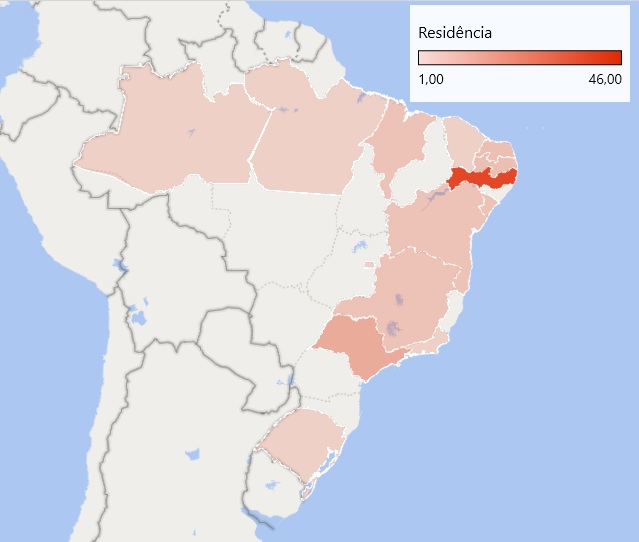
\includegraphics[width=12cm]{images/residencia.jpg}
    \caption{Mapa de densidade demográfica dos participantes}
    \label{fig:residencia}
\end{figure}


\begin{table}[H]
\centering
\caption{Local onde residem os participantes}
\label{tab:residencias}
\begin{tabular}{|c|c|}
\hline
UF            & QUANTIDADE \\ \hline
\rowcolor[HTML]{FFCCC9} 
AM            & 1             \\ \hline
\rowcolor[HTML]{FFCCC9} 
PA            & 1             \\ \hline
\rowcolor[HTML]{FFFC9E} 
BA            & 2             \\ \hline
\rowcolor[HTML]{FFFC9E} 
CE            & 1             \\ \hline
\rowcolor[HTML]{FFFC9E} 
MA            & 2             \\ \hline
\rowcolor[HTML]{FFFC9E} 
PB            & 3             \\ \hline
\rowcolor[HTML]{FFFC9E} 
PE            & 45            \\ \hline
\rowcolor[HTML]{FFFC9E} 
RN            & 3             \\ \hline
\rowcolor[HTML]{FFFC9E} 
SE            & 2             \\ \hline
\rowcolor[HTML]{9AFF99} 
DF            & 1             \\ \hline
\rowcolor[HTML]{CBCEFB} 
MG            & 1             \\ \hline
\rowcolor[HTML]{CBCEFB} 
RJ            & 1             \\ \hline
\rowcolor[HTML]{CBCEFB} 
SP            & 11            \\ \hline
\rowcolor[HTML]{34CDF9} 
RS            & 1             \\ \hline
\rowcolor[HTML]{C0C0C0} 
Estrangeiro   & 2             \\ \hline
Não Declarado & 1             \\ \hline
TOTAL         & 78            \\ \hline
\end{tabular}
\end{table}

\chapter{Resultados}
\label{chp:resultados}

\section{Estudo 1 - Pesquisa Qualitativa}

As entrevistas semiestruturadas, após terem seus dados coletados com a finalidade de capturar as percepções dos participantes, motivações e sentimentos no tocante a participação dos eventos de hackathon, passaram pelo processo de codificação, categorização, redução e comparação dos dados. Este processo extraiu quatro temáticas principais, os quais serão descritas mais adiante
\begin{enumerate}
    \item Ambientação 
    \item Percepção dos Regulamentos
    \item Sentimentos sobre os Regulamentos
    \item Confiança nas Hackathons
\end{enumerate}



\subsection{Ambientação}
% no tocante rsrs
Aqui o participante se ambienta no tocante a motivação para participar das hackathons e o tipo de hackathon que foi abordada.

Os que \textbf{cederam a sua PI} tem como principal motivação o desafio, a vontade de aprender novidades em um curto espaço de tempo, junto ao desafio veio a questão financeira, pois de acordo com o entrevistado 2 "é unir o útil ao agradável".

Também foi entendido qual o tipo de eventos que eles participaram conforme descrito por eles

\begin{quote}
    "O primeiro era da prefeitura de Recife, era um hackathon onde basicamente você criava a plataforma e a solução ficava pra prefeitura pra ela dar continuidade. O segundo era um hackathon que também tinha participação da prefeitura, mas não tinha participação direta, era mais um apoiador, e essa solução, eles lhe davam a solução pra que depois você continuasse sob a supervisão deles"
    
    \flushright Entrevistado 1
\end{quote}

\begin{quote}
    "As hackathons que participei eram mais do ramo empresarial. Todas elas eram sobre criar algum tipo de solução para um problema"
    
    \flushright Entrevistado 2
\end{quote}

Já os participantes que \textbf{não cederam sua PI} se destacam por terem opiniões um pouco antagônicas no tocante a motivação para participar dos eventos. A entrevistada 3 dá preferência ao aprendizado em um curto espaço de tempo, enquanto o entrevistado 4 dá preferência a premiação do evento.

\begin{quote}
    "Eu sempre observei muito que em hackathons a galera aprende muita coisa, vivencia muita coisa em pouco tempo. É uma oportunidade muito boa de aprender novas ferramentas e vivenciar coisas novas. E eu estou acostumada a experiências novas."
    \flushright Entrevistada 3
\end{quote}

\begin{quote}
    "O dinheiro (risos), o prêmio "
    \flushright Entrevistado 4
\end{quote}

Ambos participaram de hackathons empresariais, enquanto o entrevistado 4 também participou de uma hackathon governamental.

\subsection{Percepção dos Regulamentos}

Foi possível entender a percepção dos participantes quanto ao entendimento sobre PI e captar a importância nos regulamentos sobre o assunto. Sobre o entendimento, cada um deu a sua opinião conforme \autoref{tab:entendimento-PI}


\begin{table}[H]
\centering
\caption{Entendimento dos entrevistados sobre PI}
\label{tab:entendimento-PI}
\begin{tabular}{l|p{12,5cm}}
Entrevistado 1 &
  "PI é basicamente, você tem uma ideia, alguma coisa que não é física ainda e você tem propriedade sobre ela por que você foi o criador ou você teve uma grande participação sobre ela. E você tem, tipo, alguma autoridade sobre ela" \\
Entrevistado 2 &
  "Eu entendo que PI tem a ver com coisas que eu criei em determinado espaço e se dá a quem eu estou contatado a minha empresa [nome da empresa], tudo o que eu produzo relacionado ao software são PI dela, então o que eu entendo por PI é isso, alguma coisa que eu crio, mas dependendo de quem eu estou empregado ela é coisa minha ou não" \\
Entrevistado 3 & "eu entendo que seja uma ideia que você teve com o nome de propriedade intelectual, onde a ideia partiu de você." \\
Entrevistado 4 & "Que você meio que tem a sua ideia e ela é sua"                                                                  
\end{tabular}
\end{table}



Quando indagados sobre a percepção deles quanto a importância e o nível de prioridade dados pelas empresas organizadoras dos eventos de hackathon sobre propriedade intelectual. 
Todos os participantes percebem uma objetividade dos organizadores em focarem nos resultados, em alguns casos o assunto passa um pouco despercebido, conforme pode ser visto na \autoref{tab:importancia-prioridade-PI}.

\begin{table}[H]
\centering
\caption{Qual a sua percepção sobre a importância e o quanto a organização do evento dá prioridade com relação aos direitos sobre PI?}
\label{tab:importancia-prioridade-PI}
\begin{tabular}{l|p{12,5cm}}

Entrevistado 1 &
  "nesses dois hackathons que participei foram bem diferentes um do outro, mas ambos tinham participação direta da “empresa” ou do órgão que ele tava organizando. Acho isso um pouco ruim, no começo pode ser bom por que ajuda, mas é um pouco ruim por que, o que eu vejo, é basicamente uma forma barata de mão de obra. É você simplesmente arrumar uma solução que demandaria vários especialistas e jogar pra vários estudante e pessoas que querem dinheiro e você simplesmente pagar muito pouco pra te r um início de solução pra que você pague muito menos pra ter uma equipe pra desenvolver aquilo. Por que toda parte de ideação e pesquisa já tá feita, já tá validada. É você pular uma etapa de forma barata, pra empresa é uma solução ideal, é muito bom isso, agora pras pessoas pode ser que não seja uma coisa muito boa. Eu não vejo como uma coisa muito boa" \\
Entrevistado 2 &
  "A maioria das hackathons que participei a PI não eram um tópico abordado, a gente nunca teve que assinar contrato ou algo do tipo. Exceto numa hackathon que participeri da Qualcomm, foi a primeira hackathon da Qualcomm aqui em Recife. E a gente assinou algum contrato a ver, não necessariamente sobre PI, mas sobre confidencialidade e alguma coisa relacionada com o que a gente produzisse lá seria propriedade da Qualcomm. Eu já ouvi falar de alguns eventos que a pessoa participou e a propriedade cultural era daquele evento." \\
Entrevistado 3 &
  "Quando empresas patrocinam o eventos elas focam muito no produto final e não nessa parte de “ah você teve uma ideia e isso vai ser usado por uma pequena quantia ou talvez nada por isso” {[}...{]} elas normalmente só se importam com o produto final, nem tanto a ideia. Acho que não há tanto respeito quanto a isso" \\
Entrevistado 4 &
  "Infelizmente a gente descobre coisas que não são tão óbvias pra eles e infelizmente nem todo mundo é recompensado no final, e meio que as ideias vão diretamente pras pessoas que organizaram o hackathon. Basicamente é isso {[}...{]} ele não recompensa todos os participantes como deveria"
\end{tabular}
\end{table}

Foi perguntado o que o participante considera como prioridade ao ler o regulamento. Onde deveria enumerar de 1 a 5 onde 1 é o mais importante e 5 é o menos importante, dentre os seguintes critérios; Critério de avaliação, premiação, direitos à propriedade intelectual, organização da equipe, programação; A exceção do entrevistado 2 que deu notas a partir de cinco de forma decrescente, conforme pode ser visto na \autoref{tab:ranking-PI}. 


\begin{table}[H]
\centering
\caption{Enumerando de 1 a 5 onde 1 é o mais importante e 5 o menos importante, quais critérios você considera como mais importante dentre estes? Critério de avaliação, premiação, direitos à PI, organização da equipe, programação.}
\label{tab:ranking-PI}
\begin{tabular}{l|p{12,7cm}}
Entrevistado 1 &
  "Critério de avaliação eu vejo como 5, menos importante. Premiação 1, basicamente eu só vou pra uma hackathon pra ganhar alguma coisa {[}...{]}. Direito a PI eu boto 3, por que dependendo da premiação pode ser que eu ligue ou não de ficar com a ideia, e depende até da ideia. Organização de equipe eu boto como 2, equipe é muito importante em hackathon, eu sofri muito no segundo por que só tinha 2 pessoas e o resto das equipes eram tudo 5 e o resto das equipes passaram muito à frente da gente que só tinha 2 pessoas. {[}...{]}. É importante, no primeiro por exemplo ele foi bem desorganizado e atrapalhou pra caramba. Apesar de ter conseguido o segundo lugar, ele atrapalhou pra caramba qualquer coisa." \\
Entrevistado 2 &
  "(Avaliando por notas de 5 pra baixo) Acredito que critério de avaliação, ele é muito importante, é importante deixar isso claro para os competidores, então é 5. {[}...{]} Premiação é importante, mas não demais, o reconhecimento por ter ganhado é mais importante, acredito que daria um 3 ou 4 pra isso, 3 e meio. Direito a PI dou 4, mas porque, se a gente tiver usando algum tipo de software algum tipo de hardware, qualquer ferramenta dada pela empresa acredito que a empresa tem direito a aparte do que eu fiz. {[}...{]} Organização da equipe muito importante, eu dou um 4, não é fundamental, mas é muito importante. E a programação, muito importante, 5. Por que se a programação foi muito ruim, por exemplo, você vem nesse sábado e 'ahh' na outra semana você vem de novo, não tem sentido isso." \\
Entrevistado 3 &
  "A premiação é muito importante, visto que atualmente a gente considera que tempo é dinheiro. {[}...{]} A premiação é muito importante como fator de reconhecimento pelo seu esforço. O segundo o direto a propriedade intelectual, é importante por que {[}...{]} como eu disse, a empresa vem pegando o produto, com o esforço enorme feito e você não vai ter direito a nada e você deu aquela ideia e ponto tchau. O critério de avaliação é importante pra você saber de que se trata a hackathon. {[}...{]} Depois a programação, normalmente é a mesma, então é a última, é a que menos importa, é muito parecido, sabe?.. Em penúltimo a formação da equipe." \\
Entrevistado 4 &
  "O mais importante é programação, teve um hackathon que eu fiz e só tinha mentoria o tempo inteiro, você tinha 2h pra fazer alguma coisa, foi terrivelmente ruim. Critério de avaliação {[}...{]} direito a propriedade, premiação e organização de equipe... organização de equipe ficaria em penúltimo e direito a PI ficaria em último. Pois meio que você já sabe que tá vendendo a ideia"
\end{tabular}
\end{table}

Também foi perguntado o quão claro fica os direitos à PI do conteúdo do regulamento para os eventos em que participaram. Para todos os participantes que cederam a PI não há clareza ou há pouca clareza quanto aos direitos à PI daquele evento. Para os que não cederam a PI somente o entrevistado 4 enxerga que no regulamento fica bem explícito para quem fica os direitos à PI daquela hackathon conforme pode ser visto na \autoref{tab:clareza-PI}



\begin{table}[H]
\centering
\caption{De acordo com o regulamento que é proposto pelo evento, o quão claro fica os direitos à propriedade intelectual do conteúdo feito por você naquele evento?}
\label{tab:clareza-PI}
\begin{tabular}{l|p{12,5cm}}
Entrevistado 1 &
  "{[}...{]} nas duas hackathons que participei eu li os dois editais e em nenhum deles ficou claro se você ia levar alguma coisa depois. O único que deixou transparecer um pouquinho foi o segundo que eles disseram que você vai ter o direito de trabalhar com eles na sua ideia depois {[}...{]}" \\
Entrevistado 2 &
  "Honestamente não muito. Muitas das hackathons não deixa claro o suficiente... deixa claro a premiação, tal.{[}...{]} o que eu lembro dos editais é que eles não falavam sobre PI no conteúdo, realmente não lembro. Tenho quase certeza que não existia nos editais"" \\
Entrevistado 3 & "Lembro de ter lido algo que seria usado pela empresa e lembro de assinar algo relacionado aos meus direitos." "{[}...{]} tem total brecha" \\
Entrevistado 4 & "Fica claro que não é meu, geralmente todo conteúdo produzido numa hackathon, é da hackathon, meio que você só produz pra eles"            
\end{tabular}
\end{table}

Quando perguntado sobre a outra hackathon o entrevistado 4 respondeu que: \begin{quote}
    "Você teria preferência caso a ideia fosse pra frente, mas nada do tipo, você vai ganhar tantos porcento da participação" 
\end{quote}

Assim, abrindo espaço para parcerias futuras, mas sem especificar melhor como ela seria continuada.







\subsection{Sentimento sobre os Regulamentos}

Buscou-se entender o que o participante sentia com relação aos seus direitos à PI quando participava de uma hackathon. Assim foi perguntado aos participantes qual o sentimento deles com relação ao seu direito à PI em um evento de hackathon. 
%COMENTAR SOBRE
como é mostrado na \autoref{tab:sente-respeito}

%%%% PERGUNTA 10
\begin{table}[H]
\centering
\caption{Quando você participa de um evento de hackathon, o que você sente a respeito do seu direito à propriedade intelectual?}
\label{tab:sente-respeito}
\begin{tabular}{l|p{12,5cm}}
Entrevistado 1 &
  "{[}...{]} eu vejo as coisas de como 'eu posso lucrar com isso'.  Nessa hora eu sinto que estou perdendo uma vantagem, perdendo dinheiro de uma solução que eu poderia estar criando sozinho. Algo que eu poderia tá explorando por fora e sem a interferência de outras pessoas que limitam aquilo. {[}...{]} Aí eu sinto que essa minha parte do meu direito à propriedade intelectual está totalmente limitada" \\
Entrevistado 2 &
  "{[}...{]} eu sinto que tenho direito, tanto que a minha startup, {[}...{]} nasceu de uma hackathon, mas a gente não usou as ferramentas deles, a gente usou outras ferramentas. Mas os meus direitos sobre  à PI, embora nunca tenha sido me dito, eu sempre senti que tinha a liberdade sobre o que eu criava, então, nunca me pararam, me falaram, ‘ahh você tá devendo x ou y pra gente’, não! Eles nunca falaram isso. Tudo o que fiz na hackathon, ou ficava na hackathon ou não perguntaram depois" \\
Entrevistado 3 &
  "Sinceramente, nunca havia parado pra pensar sobre os meus direitos, eu vou como o pensamento de aprender e ganhar, {[}...{]} mas nunca tinha parado para pensar sobre os meus direitos não" \\
Entrevistado 4 &
  "Como a pessoa escolhe participar se quiser, sim é respeitado. O direito você que vai dizer se vai querer ou não"
\end{tabular}
\end{table}




%%%% PERGUNTA 11
Quando indagados se venderiam a solução encontrada, todos os participantes não hesitariam em vender, porém o valor varia muito de acordo com a sua implementação como pode ser visto na \autoref{tab:vender-solucao}

\begin{table}[H]
\centering
\caption{Venderia a sua solução? Se sim por quanto? }
\label{tab:vender-solucao}
\begin{tabular}{l|p{12,5cm}}
Entrevistado 1 & "Venderia, por muito mais do que o pessoal dá."                                                            \\
Entrevistado 2 & "Pelas minhas ideias pelo menos uns 100 mil, não pelo produto, mas pela ideia, pelo produto seria menor"   \\
Entrevistado 3 & "Se eu visse que tem mercado e pudesse comercializar eu venderia, se alguém tivesse disposto a pagar eu aceito" \\
Entrevistado 4 & "Depende do quão boa é a solução, tem solução que seria o prêmio e tem outras que poderia ser milionária."
\end{tabular}
\end{table}

%%%% PERGUNTA 12

Támbem foram indagados sobre as diferenças de como foram abordadas o tópico sobre PI em outras hackathons, conforme pode ser visto na \autoref{tab:diferencas}.
A entrevistada 3 participou de apenas uma hackathon, por isso não respondeu a pergunta.

\begin{table}[H]
\centering
\caption{Qual a principal diferença com relação a propriedade intelectual dentre as outras hackathons que participou? Tem alguns exemplos negativos? }
\label{tab:diferencas}
\begin{tabular}{l|p{12,5cm}}
Entrevistado 1 &
  "{[}...{]} não é muito claro quando fala de PI, e também não é muito claro o quanto eles iriam lucrar nisso e se eu teria participação nisso, já que a ideia foi minha. Não é muito claro até onde vai a minha parte de consultoria, por que no final das contas a gente não documenta nada em hackathons." \\
Entrevistado 2 & "Nenhuma delas falou muito, a única que realmente falou foi a Qualcomm, eles realmente mencionaram"            \\

Entrevistado 4 & "As hackathons empresariais geralmente querem a sua ideia, pra privatizar do que as da prefeitura, do governo"
\end{tabular}
\end{table}


\subsection{Confiança nas Hackathons}

Na última bateria de questões os participantes puderam discorrer um pouco sobre a confiança deles quanto aos eventos. Uma das perguntas indaga se eles deixariam de participar de uma hackathon caso o direito à PI não ficassem com eles. Como pode ser encontrado na \autoref{tab:deixaria-de-participar}.
%%%% PERGUNTA 13

\begin{table}[H]
\centering
\caption{Deixaria de participar de uma hackathon caso o direito à propriedade intelectual não ficasse com você?}
\label{tab:deixaria-de-participar}
\begin{tabular}{l|p{12,5cm}}
Entrevistado 1 & "Não, só se a premiação fosse muito ruim"                                         \\
Entrevistado 2 &
  "Com certeza, embora eu tivesse participando de um evento onde a empresa tivesse dando todo o material, toda a ferramenta, eu acredito que a minha PI que eu fiz, {[}...{]} eu não deixaria de participar fácil" \\
Entrevistado 3 &
  "Eu deixaria de participar, se não tivessse premiação coisa assim, deixaria de participar. Por que a premiação é meio que um pagamento pela sua ideia, então você tá abrindo mão da sua ideia por um valor." \\
Entrevistado 4 & "Depende do prêmio, se o prêmio for um milhão por exemplo, eu cedo sem problemas"
\end{tabular}
\end{table}



%%%% PERGUNTA 14
Também doi perguntado se eles têm confiança em ceder os códigos-fonte que criou no evento para a empresa organizadora conforme pode ser visto na \autoref{tab:confianca}.

\begin{table}[H]
\centering
\caption{Tem confiança em ceder os códigos-fonte que criou no evento para a empresa organizadora?}
\label{tab:confianca}
\begin{tabular}{l|p{12,5cm}}
Entrevistado 1 &
  "Depende do projeto, se o projeto tiver um impacto que eu sei que é muito bom pra sociedade ou eu veja muito potencial, eu não gostaria de ceder. Agora se fosse alguma solução, por exemplo, a solução que eu fiz no primeiro hackathon {[}...{]} Isso aí eu tenho pouco interesse, não seria problema se eles vão ficar ou não." \\
Entrevistado 2 &
  "Tenho, mas só depois de eu fazer um “commit” no GitHub, deixar claro pra todo mundo, provas, botar no meu Drive, tudo o que eu puder documentar, pra deixar claro aqueles códigos, tudo o que eu fiz primeiro, a eu faria, mas dependendo da empresa. {[}...{]} Depende muito da empresa, eu confio muito nas empresas de código aberto" \\
Entrevistado 3 & "Se ele me pagar daria"                                                                                                                          \\
Entrevistado 4 & "Tenho sim, eles não vão entender. {[}...{]} já que é simplesmente pra apresentar o pitch ou algo muito funcional que seja só pra demonstração."
\end{tabular}
\end{table}



%%%% PERGUNTA 15


Foi perguntado também se nos eventos os participantes sentem que o seu direito à PI são respeitados conforme pode ser visto na \autoref{tab:respeito}.


\begin{table}[H]
\centering
\caption{Nos eventos de hackathon, sente que seu direito à propriedade intelectual é respeitado?}
\label{tab:respeito}
\begin{tabular}{l|p{12,5cm}}
Entrevistado 1 &
  "Não. No primeiro, não, que foi com a prefeitura. No segundo que foi sem a interferência da prefeitura, eles respeitaram até um certo limite, eles deixaram você trabalhar, caso vencessem {[}...{]}" \\
Entrevistado 2 &
  "{[}...{]} geralmente, como não tem essa conversa sobre PI, geralmente fico assim 'talvez sim, talvez não'. Eles não deixam, claro, eu não sei se sou desrespeitado ou não, aí vira um problema" \\
Entrevistado 3 & "Nas que participei sim. {[}...{]} mas não sinto que fui roubada ou que não tinha propriedade intelectual, houve respeito sim." \\
Entrevistado 4 & "Sim"                                                                                                                          
\end{tabular}
\end{table}





















\section{Estudo 2 - Pesquisa Quantitativa}

Após recolhimento das 78 respostas obtidas dos participantes do estudo, foram plotados gráficos e tabelas para representar visualmente os dados coletados. O questionário completo encontra-se no \autoref{ap:questionario} do presente trabalho. Os dados coletados para identificação demográfica da amostra,  referentes as perguntas 2, 3, 4 e 5 do questionário, encontram-se na \autoref{tab:dados-demo} e na \autoref{fig:residencia} do capítulo que trata da Metodologia do Estudo 2 – Estudo Quantitativo (seção Amostra).


O questionário interroga sobre a quantidade de hackathons em que o participante participou, com média de participações de aproximadamente 3,99 por pessoa (desvio padrão = 6,61). %Pergunta 6

Também foram indagados se os participantes leem os regulamentos das hackathons que participaram, o resultado está registrado no gráfico da \autoref{fig:le-regulamento}. % pergunta 7

\begin{figure}[H]
    \centering
    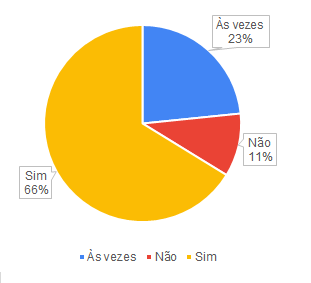
\includegraphics{images/Grafico-leitura-regulamentos.png}
    \caption{Você lê os regulamentos das hackathons que participa?}%pergunta 7
    \label{fig:le-regulamento}
\end{figure}


Foi questionado sobre o que o participante acha mais interessante ao ler o regulamento de uma hackathon. Essa foi uma pergunta facultativa, a qual recebemos 27 (vinte e sete respostas), algumas com duas ou mais propostas de tópicos, destrinchando-as foi totalizado 68 (sessenta e oito) tópicos. Por ser uma pergunta aberta, tivemos que agrupar os dados, pois o Google Forms não consegue agrupar em caso de divergência, muitas vezes mínima, com relação à grafia da palavra digitada. %Pergunta 8
Algumas ressalvas devem ser pontuadas, como a junção de propriedade industrial em propriedade intelectual, alguns critérios como "entender como funciona", "todos", "objetivos", foram tratados como generalidades.

\begin{figure}[H]
    \centering
    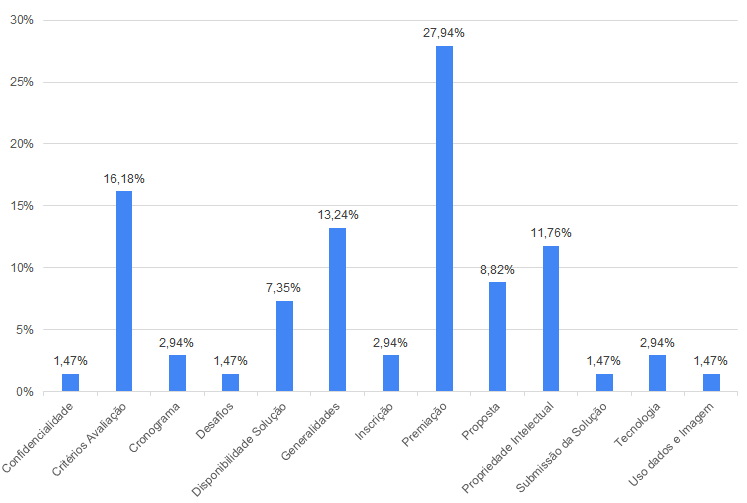
\includegraphics[width=0.8\textwidth]{images/topico-interessante.png}
    \caption{Qual tópico você acha interessante ao ler um regulamento de Hackathon?}% pergunta 8
    \label{fig:topico-interessante}
\end{figure}


Foi proposto um ranking dentre cinco tópicos aos participantes, onde eles teriam que categorizar o quanto eles consideram os seguintes tópicos ao ler o regulamento de uma hackathon do mais relevante ao menos relevante: Programação do Evento, direitos à Propriedade Intelectual, premiação,formação da equipe, premiação e critério de avaliação. Conforme pode ser visto na \autoref{fig:ranking}. %pergunta 9

\begin{figure}[H]
    \centering
    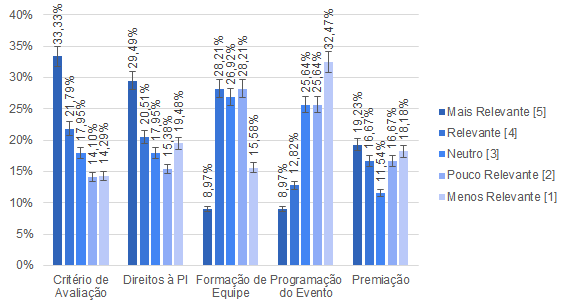
\includegraphics[width=0.8\textwidth]{images/ranking.png}% talvez tenha q melhorar a figura
    \caption{De 1 a 5, sendo 5 o MAIS relevante e 1 o MENOS relevante, o quão relevante você considera os seguintes tópicos ao ler o regulamento de uma Hackathon?}
    \label{fig:ranking}
\end{figure}%pergunta 9



Foi perguntado o quão importante é para o participante, no regulamento, o tópico de propriedade intelectual. Conforme pode ser visto o gráfico contido na \autoref{fig:importancia}.

\begin{figure}[H]
    \centering
    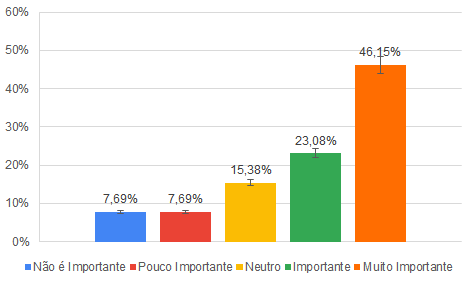
\includegraphics{images/importante.png}
    \caption{O quão importante é pra você no Regulamento o tópico de Propriedade Intelectual?}
    \label{fig:importancia}
\end{figure}


A pergunta 11 do questionário tentou avaliar a clareza dos regulamentos quanto à quem fica os direitos à propriedade intelectual do conteúdo feito pelo participante nas hackathons. De acordo com a \autoref{fig:clareza}

\begin{figure}[H]
    \centering
    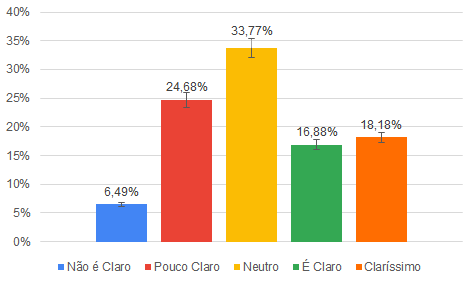
\includegraphics{images/clareza.png}
    \caption{O regulamento é sempre claro para quem fica os direitos à propriedade intelectual do conteúdo feito por você naquele evento?}
    \label{fig:clareza}
\end{figure}

A 12ª (décima segunda) pergunta do questionário foi pedido ao participante para afirmar se geralmente cedem os seus direitos à Propriedade Intelectual numa hackathon. 53,6\% afirmaram que cedem sim, os seus direitos, os outros 45,4\% afirmaram que não cedem os direitos.

Objetivamente foi perguntado se o participante venderia o protótipo da solução desenvolvida no hackathon. Obtivemos massivamente 90\% afirmando que venderia a solução e apenas 10\% não venderia.

Relacionada à pergunta anterior, foram sugeridos valores pelo qual o participante venderia sua solução, conforme pode ser visto na \autoref{fig:valor-sugerido}

\begin{figure}[H]
    \centering
    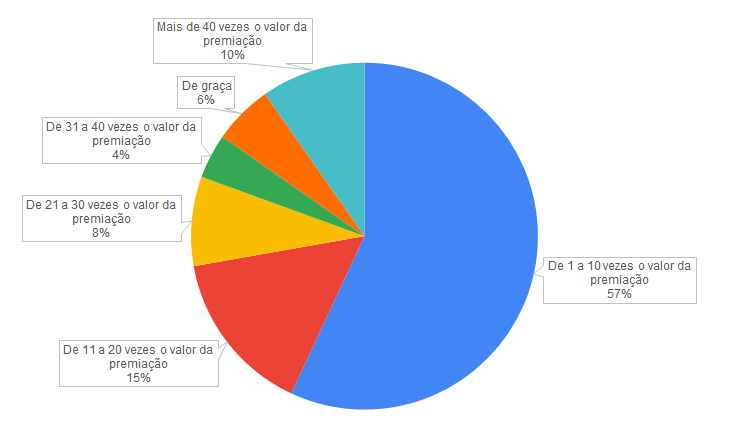
\includegraphics[width=0.7\textwidth]{images/Grafico-valor-venda-solucao.png}
    \caption{Venderia o protótipo da solução desenvolvida no hackathon?}
    \label{fig:valor-sugerido}
\end{figure}

%   pergunta 15
Também foi perguntado se o participante deixaria de participar de uma hackathon caso não ficassem com os direitos à propriedade intelectual. Em sua maioria, 55,9\% afirmam que deixaria de participar do evento caso o direito não pertencesse à pessoa. Os outros 44,1\% pessoas não deixariam de participar do evento.

Dentre os participantes, 49,35\% afirmaram que já abriu mão de propriedade intelectual em algum hackathon, enquanto 50,65\% afirmam não terem aberto mão. %pergunta 16

Os participante indagaram sobre o quanto a PI é respeitada nos eventos, assim como o interesse em saber ou entender sobre os direitos que eles têm sobre a PI conforme podem ser vistos nas \autoref{fig:respeito} e \autoref{fig:interessante-entender} abaixo. %pergunta 17 e 18

\begin{figure}[H]
    \centering
    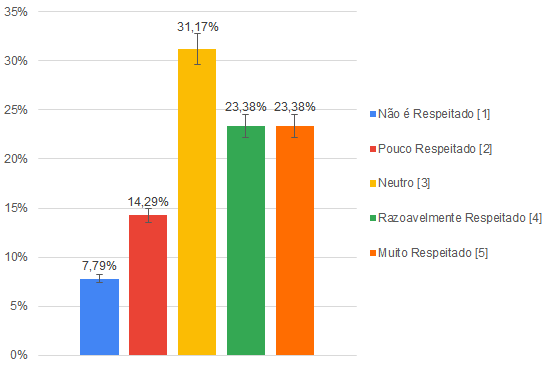
\includegraphics[width=0.8\textwidth]{images/PIrespeitada.png}
    \caption{Nos eventos em que participou, o quanto você sente que seu direito à propriedade intelectual é respeitado?}
    \label{fig:respeito}
\end{figure}



\begin{figure}[H]
    \centering
    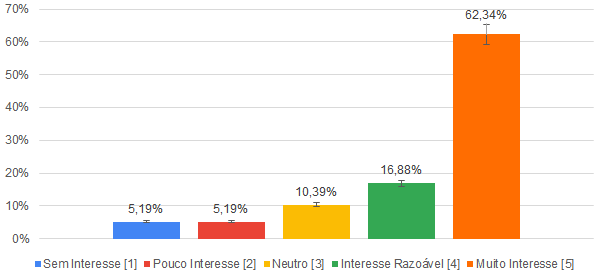
\includegraphics[width=0.8\textwidth]{images/interesseAprender.png}
    \caption{O quão interessante você acha saber/entender sobre a propriedade intelectual e seus direitos sobre ela?}
    \label{fig:interessante-entender}
\end{figure}



A penúltima pergunta indaga sobre a confiança em ceder os códigos-fonte após o evento para a empresa organizadora, onde 49,35\% afirmam não confiarem, enquanto 50,65\% asseguram confiança em ceder os códigos-fonte à empresa organizadora após o evento.

\chapter{Discussão}
\label{chp:Discussão}

A empolgação e entusiasmo levam jovens e adultos a participarem de eventos de hackathons \citep{zukin2017hackathons}, os mesmos tendem muitas vezes a negligenciar certos aspectos, tais como bem estar ou mesmo direitos à propriedade intelectual como \citet{zukin2017hackathons} descrevem, pois muitas vezes existe uma certa efevercência e empolgação, além de uma grande interação que os levam a negligenciarem esses pontos inerentes a eles \citep{zukin2017hackathons} \citep{pompa2013allen}. Por sua vez, muitas empresas aproveitam essa situação de fragilidade para monetizar os códigos dos participantes. \citep{pompa2013allen}

Para entender melhor a situação de como os participantes de hackathons veem e compreendem sobre os seus direitos ao ingressarem em uma competição, foi realizado este estudo. 


%% PERCEPÇÂO ESTUDO QUALITATIVO
Alguns pontos do estudo qualitativo, entender a percepção em alguns tópicos abordados como a percepção do entendimento sobre PI pelos regulamentos das competições que eles participaram. Onde os participantes entendem que PI é algo inerente a eles, onde eles sabem que aquela determinada ideia pertence a eles. Quanto ao nível de prioridade e a importância que a organização do evento dá ao tema os entrevistados não veem com clareza que o tema dos direitos à PI é bem abordado nos regulamentos. Eles têm a impressão que as empresas focam muito no produto final e não nesses tópicos de tamanha relevância para os participantes.

%%%%%%%%% RANKING
Foi pedido para os entrevistados enumerarem de 1 a 5 onde 1 é o mais importante e 5 o menos importante, quais critérios eles consideram como mais importante dentre os seguintes: Critério de avaliação, premiação,direitos à propriedade intelectual, organização da equipe, programação. Foi visto que todos tiveram uma certa divergência quanto aos principais pontos, onde foi visto que os entrevistados 1 e 3 escolheram o tópico de premiação como mais importante. Diferente do visto na pesquisa quantitativa que coloca como mais importante o tópico de critério de avaliação e uma pouca relevância ao tópico de premiação.


Também perguntados sobre a clareza quanto a quem fica os direitos à PI do conteúdo feito por eles naquele evento, os entrevistados não encontraram clareza quanto ao conteúdo sobre PI. O entrevistado 2 fala: \begin{quote}
    "Muitas das hackathons não deixa claro o suficiente... deixa claro a premiação, tal.[...]". 
\end{quote}
Somente o entrevistado 4 viu uma certa clareza, porém de forma negativa \begin{quote}
    "Fica claro que não é meu, geralmente todo conteúdo produzido numahackathon, é da hackathon[...]". 
\end{quote}

Quanto ao sentimento dos participantes em relação ao respeito do direto à PI há divergências entre os participantes de ambas as categorias, levando a abrir cada vez mais o debate. Pelo lado dos que \textbf{cederam PI}, o entrevistado 1 sente que o seu direito está sendo colocado de forma limitada, pois o pensamento é um pouco mais voltado ao lucro das ideias, enquanto o entrevistado 2 tem a percepção de mais liberdade quanto ao respeito dos seus direitos. Já pelo lado dos que \textbf{não cederam PI} a entrevistada 3 "não parou pra pensar sobre o assunto", enquanto o entrevistado 4 nota que o direito à PI vai ser respeitado de acordo com a escolha do participante em entrar ou não na competição. \begin{quote}
    "Como a pessoa escolhe participar se quiser, sim é respeitado.  O direito você que vai dizer se vai querer ou não".
\end{quote}

Quando perguntados se eles venderiam ou não eles foram categóricos afirmando que venderiam, ambos os entrevistados que \textbf{cederam PI} venderiam por um valor acima do oferecido no regulamento da hackathon. Os entrevistados que \textbf{não cederam PI} venderiam com ressalvas, principalmente no sentido de analisar melhor as propostas do mercado.

Ao serem perguntados sobre as principais diferenças encontradas nos regulamentos dentre as hackathons que participaram, ambos os participantes que \textbf{cederam PI} falam da falta de clareza entre os regulamentos, enquanto o entrevistado 4 focou no objetivo de privatização das ideias pelas hackathons do tipo empresariais.

Ao medir a confiança dos participantes com relação às hackathons, perguntamos se os entrevistados deixariam de participar de uma hackathon caso o direito à propriedade intelectual não ficasse com eles. A premiação seria o ponto chave para que eles decidissem não participar, como a entrevistada 3 pontua \begin{quote}
    "Por que a premiação é meio que um pagamento pela sua ideia,então você tá abrindo mão da sua ideia por um valor".
\end{quote}

Quando perguntados se teriam confiança em ceder os códigos-fonte que criaram para a empresa organizadora os participantes que cederam PI foram mais conservadores, cederiam com menos impedimentos dependendo da relevância ou dependendo do impacto que a solução poderia causar, diferente dos participantes que não cederam PI, que se mostram mais abertos cederiam com mais facilidade.

Ao serem indagados se nos eventos de hackathon, sentem que o seu direito à propriedade intelectual é respeitado, os entrevistados que \textbf{cederam PI} não sentem ou possuem dúvidas quanto ao respeito dado pelas organizadoras do evento ao seu direito à PI. Contrariando os participantes que \textbf{não cederam PI} que afirmam que houve respeito sim, aos seus direitos à PI.

















%% PERCEPÇÂO ESTUDO QUANTITATIVO

Também foi realizada uma pesquisa quantitativa visando entender melhor os pontos de vista de forma mais ampla. Assim, no presente estudo pudemos destrinchar as respostas das perguntas realizadas.

No que se diz respeito a leitura dos regulamentos 66\% responderam que leem, mostrando que há um interesse em entender em que tipo de evento estão participando. 

Questionando os participantes para entender qual tópico eles acham mais interessante, pudemos perceber que quase em sua maioria os participantes buscam o tópico de \textbf{premiação}, com 27,94\%, por achar interessante saber o quanto podem ser estimulados participando do evento. \textbf{Critério de avaliação} ficou em segundo lugar com cerca de 16,18\%, o que nos leva a refletir que o participante quer entender como chegar nessa premiação.

%ranking polêmico
Na pergunta onde os entrevistados enumeraram de 1 a 5 onde 1 é o mais importante e 5 o menos importante, quais critérios eles consideram como mais importante dentre os seguintes: Critério de avaliação, premiação,direitos à propriedade intelectual, organização da equipe, programação, os participantes elegeram o tópico de critério de avaliação como o tópico mais importante ao ler o regulamento, onde o mesmo é relevante para 55,12\%, enquanto o tópico de direitos à PI é relevante para 50\% dos participantes, formação de equipe é relevante para 37,18\%, programação do evento 21,27\% e a premiação é relevante para 36,30\% dos entrevistados.
%%%%%%%%%%%%%%%%%%%%%%%%%%%%%%

Quando perguntado o quão importante é o tópico sobre PI nos regulamentos das hackathons, essa que foi uma pergunta com resposta em formato da escala de Likert, em sua maioria, cerca de 69,23\% dos participantes afirmaram ser importante enquanto outros 30,76\% se mostraram neutros ou não consideram importante o tópico.

Com relação a clareza, 35,06\% afirmaram que o regulamento deixa claro pra quem fica os direitos à PI enquanto 64,94\% declararam neutralidade ou a não clareza dos regulamentos.

Cerca de 53,6\% afirmaram que cedem os direitos à PI numa hackathon. O que nos leva a pergunta quanto a clareza dada nos regulamentos conforme visto no tópico anterior. Como não há clareza nos regulamentos, como entender a cessão ou não cessão dos direitos à PI em um determinado evento? Com quem realmente fica? 

Assim como foi visto, 90\% dos participantes afirmam que venderiam o protótipo da solução. E como pode ser visto na pergunta seguinte, o valor a ser pago, de acordo com 57\% dos entrevistados seria de 1 a 10 vezes o valor da premiação, 6\% doariam a solução enquanto outros 37\% venderiam o protótipo por um valor no mínimo 11 vezes o valor da premiação, assim corroborando com os entrevistados da pesquisa qualitativa em que apenas um dos entrevistados venderia a solução por preços extremamente acima dos valores propostos pelas organizações das hackathons.

Em sua maioria, os participantes, com cerca de 55,9\%, deixaria sim, de participar de uma hackathon caso o direito à PI não ficasse com ele naquele evento. Assim como 49,35\% afirmaram que já abriu mão de PI em algum hackathon, enquanto 50,65\% afirmam não terem aberto mão. O resultado com pouca disparidade leva a crer na desconfiança dos participantes quanto a clareza nos regulamentos vistos em tópicos anteriores.

Quando indagados sobre o que o participante sentem quanto ao respeito os direitos à PI nos eventos 46,76\% sentem que são respeitados enquanto outros 53,25\% se mostram neutros ou não sentem que seus direitos são respeitados.

Também foi visto o quão interessante o participante acha saber ou entender sobre o assunto de PI, onde massivamente 79,22\% veem com bons olhos e interesse no assunto, mostrando o desejo em aprender cada vez mais sobre algo de tamanha relevância. 

Por fim os participantes indagam que há dúvidas quanto a ceder ou não os códigos-fonte à empresa organizadora do evento após a hackathon, pois vemos que 49,35\% dos participantes não confiam em ceder enquanto outros 50,65\% cederiam sem problemas algum.


\section{Limitações do Trabalho}

Foi constatado ao final da pesquisa, na realizada com abordagem quantitativa que, em sua maioria, 59\% dos participantes, residem no estado de Pernambuco, mais precisamente todos residentes de municípios que fazem parte da Região Metropolitana do Recife. Assim como na pesquisa qualitativa, todos os participantes também residem em municípios que fazem parte da Região Metropolitana do Recife. Assim o escopo da pesquisa pode possuir um viés local.

\chapter{Conclusão}
\label{chp:conclusão}


Os eventos de hackathons são cercados de diversas regalias onde os participantes podem aproveitar, e muito, a sua estadia com um certo conforto, dependendo dos organizadores. Assim, muitas vezes, assuntos pertinentes ao bem estar ou relacionados aos direitos que o participante tem passam despercebidos. \citet{zukin2017hackathons} cita diversos pontos em que os participantes, em meio a empolgação do evento, negligenciam, ou lembram de forma mínima. Um deles é o tópico sobre com quem fica a PI do código produzido no evento, onde em alguns casos é dúbia a definição. \citep{steele_2013}

Como pôde ser visto nos resultados, a clareza e melhores definições nos regulamentos podem sim ajudar o participante a entender melhor o que significa a cessão ou não cessão dos direitos à PI em uma determinada hackathon. Com isso, dá-se mais liberdade ao participante de escolher ou não ceder os seus direitos. A lei brasileira é clara ao dizer a quem pertence os direitos à PI em um determinado evento, porém os regulamentos, muitas vezes mal escritos, põem em dúvida a cessão ou não dos direitos pelo participante, como já ocorreram em regulamentos bizarramente escritos\footnote{Regulamento retirado do ar, mas pode ser encontrado em: <https://docplayer.com.br/23433151-Regulamento-hackathon-gerdau-2016.html>. Acessado em 20 de mai. 2020} \footnote{Notícia pode ser encontrada em: <https://meiobit.com/86685/concurso-desenvolvedores-app-samsung-smarttv/>. Acessado em 20 de mai. 2020}.

Conforme pesquisa os participantes desejam sim, aprender mais sobre seus direitos à PI e possuem interesse no mesmo. A partir do momento em que um participante começa a compreender melhor o conceito de propriedade intelectual, os direitos que o mesmo tem ao escrever um pedaço de código, ao expor uma ideia de forma visível e fora da sua mente, o mesmo consegue escolher melhor o evento que participará, não será ludibriado por atrativos. Por isso a importância de aprender e entender os seus direitos e os direitos a um código-fonte escrito por um participante ou sua equipe.

O entendimento sobre o assunto fará com que as hackathons sejam mais acessíveis, além de garantir aos participantes liberdades de escolha, principalmente escolher ou não ceder os direitos à PI em um determinado evento. Não apenas participar do evento por uma empolgação e esquecer aquilo que pode beneficiar o participante, juntamente com a empresa patrocinadora do evento, de forma cooperativa e saudável.




\section{Trabalhos Futuros}


 Este é um trabalho que pode ser estendido amplamente, onde pode ser abordado o mesmo tema em caráter mais abrangente nacionalmente e também internacionalmente visto a quantidade restrita de estudos do assunto. Além de também abordar outros aspectos de hackathons envolvendo a provável insalubridade dos eventos.


% References

\begin{references}
  \bibliography{bibliografia}
\end{references}

% Appendix

\theappendix

% APENDICE A
\chapter{Roteiro de Entrevista}
\label{ap:entrevista}

\vspace{4mm}

\textbf{Introdução}

Esta entrevista faz parte de uma pesquisa de trabalho de graduação do pesquisador Geraldo Pereira sob a orientação do professor Kiev Gama da Universidade Federal de Pernambuco (UFPE). O objetivo é comprovar a ciência dos participantes de Hackathons sobre seus direitos à Propriedade Intelectual e suas motivações para cederem ou não tal direito. Na entrevista, procuramos entender aspectos motivacionais e percepção dos participantes de hackathons sobre o assunto.
Todas as informações fornecidas nesta entrevista serão tratadas de forma confidencial. Apenas a equipe de pesquisa terá acesso às informaões fornecidas. 
Não existem respostas corretas, seus dados são confidenciais e não serão divulgados. O intuito é extrair sua opinião a fim de contribuir para um estudo do momento atual das organizações de eventos a respeito do tema.

Sua participação nesta pesquisa é voluntária e você pode decidir por não participar ou retirar-se da pesquisa a qualquer momento. Caso você decida pela não participação, não receberá sanções ou penalidades.

Você concorda em participar desta pesquisa?

(Iniciar a gravação do áudio)
Você autoriza a gravação desta entrevista?
\vspace{4mm}

\textbf{Questões}

\textit{Dados demográficos:}

Formação:

Cargo do entrevistado(a):

Idade do entrevistado(a):

Gênero:

Naturalidade:

\vspace{4mm}
\textit{Questões sobre hackathons}

Quantidade de Hackathons realizadas:

Onde trabalha/estuda, já participou de eventos de Hackathons? 

Qual a sua motivação para participar de Hackathons?

Qual evento e o tipo de hackathon que você participou iremos abordar?
Exemplo dos tipos: Governamental, Empresarial, Recrutamento de Talentos, Criação de Novas Soluções (Melhorias na Sociedade)

\vspace{4mm} 
\textit{Questões sobre Propriedade Intelectual x Hackathon}

O que você entende por Propriedade Intelectual?

Qual a sua percepção sobre a importância (o quão importante é para você o assunto de PI na Hackathon) e o nível de prioridade dado pela organização do evento com relação aos direitos sobre propriedade intelectual?

Numa hackathon, o que você considera como prioridade ao ler o regulamento? Gostaria que enumerasse de 1 a 5 onde 1 é o mais importante e 5 o menos importante, dentre os seguintes critérios; Critério de avaliação, premiação, direitos à propriedade intelectual, organização da equipe, programação; (Se tiver outra prioridade pode acrescentar na lista e definir sua prioridade)

De acordo com o regulamento proposto, o quão claro fica  os direitos à propriedade intelectual do conteúdo feito por você naquele evento?

(Se participou de outros tipos) Conte também sobre os regulamentos de outros hackathons que participou e a clareza sobre os direitos à propriedade intelectual.

Quando participa de um evento de hackathon, o que você sente a respeito do seu direito a propriedade intelectual?

Venderia sua solução? Se sim, por quanto?

\vspace{4mm}
\textit{Para quem possui várias experiências em Hackathons}

Qual a principal diferença com relação a propriedade intelectual dentre as outras hackathons que participou? (Caso haja) Cite exemplos negativos.

\vspace{4mm}
\textit{Questões sobre Cessão de Direitos}

Deixaria de participar de uma hackathon caso o direito à propriedade intelectual não ficasse com você?

Tem confiança em ceder os códigos-fonte após o evento para a empresa organizadora?

Nos eventos, sente que seu direito à propriedade intelectual é respeitado?


\vspace{4mm}
\textit{Encerramento}

Há algo que você deseja acrescentar sobre este assunto?




%%%%%%%%%%%%%%%%%%%%%%%%%%%%%%%%%%%%%%%%%%%%%%%%%%%%%%%%%%
%%%%%%%%%%%%%%%%%%%%%%%%%%%%%%%%%%%%%%%%%%%%%%%%%%%%%%%%%%

% APENDICE B
\chapter{Termo de Consentimento da Entrevista}
\label{ap:termoConcent}
\begin{minipage}{10cm}
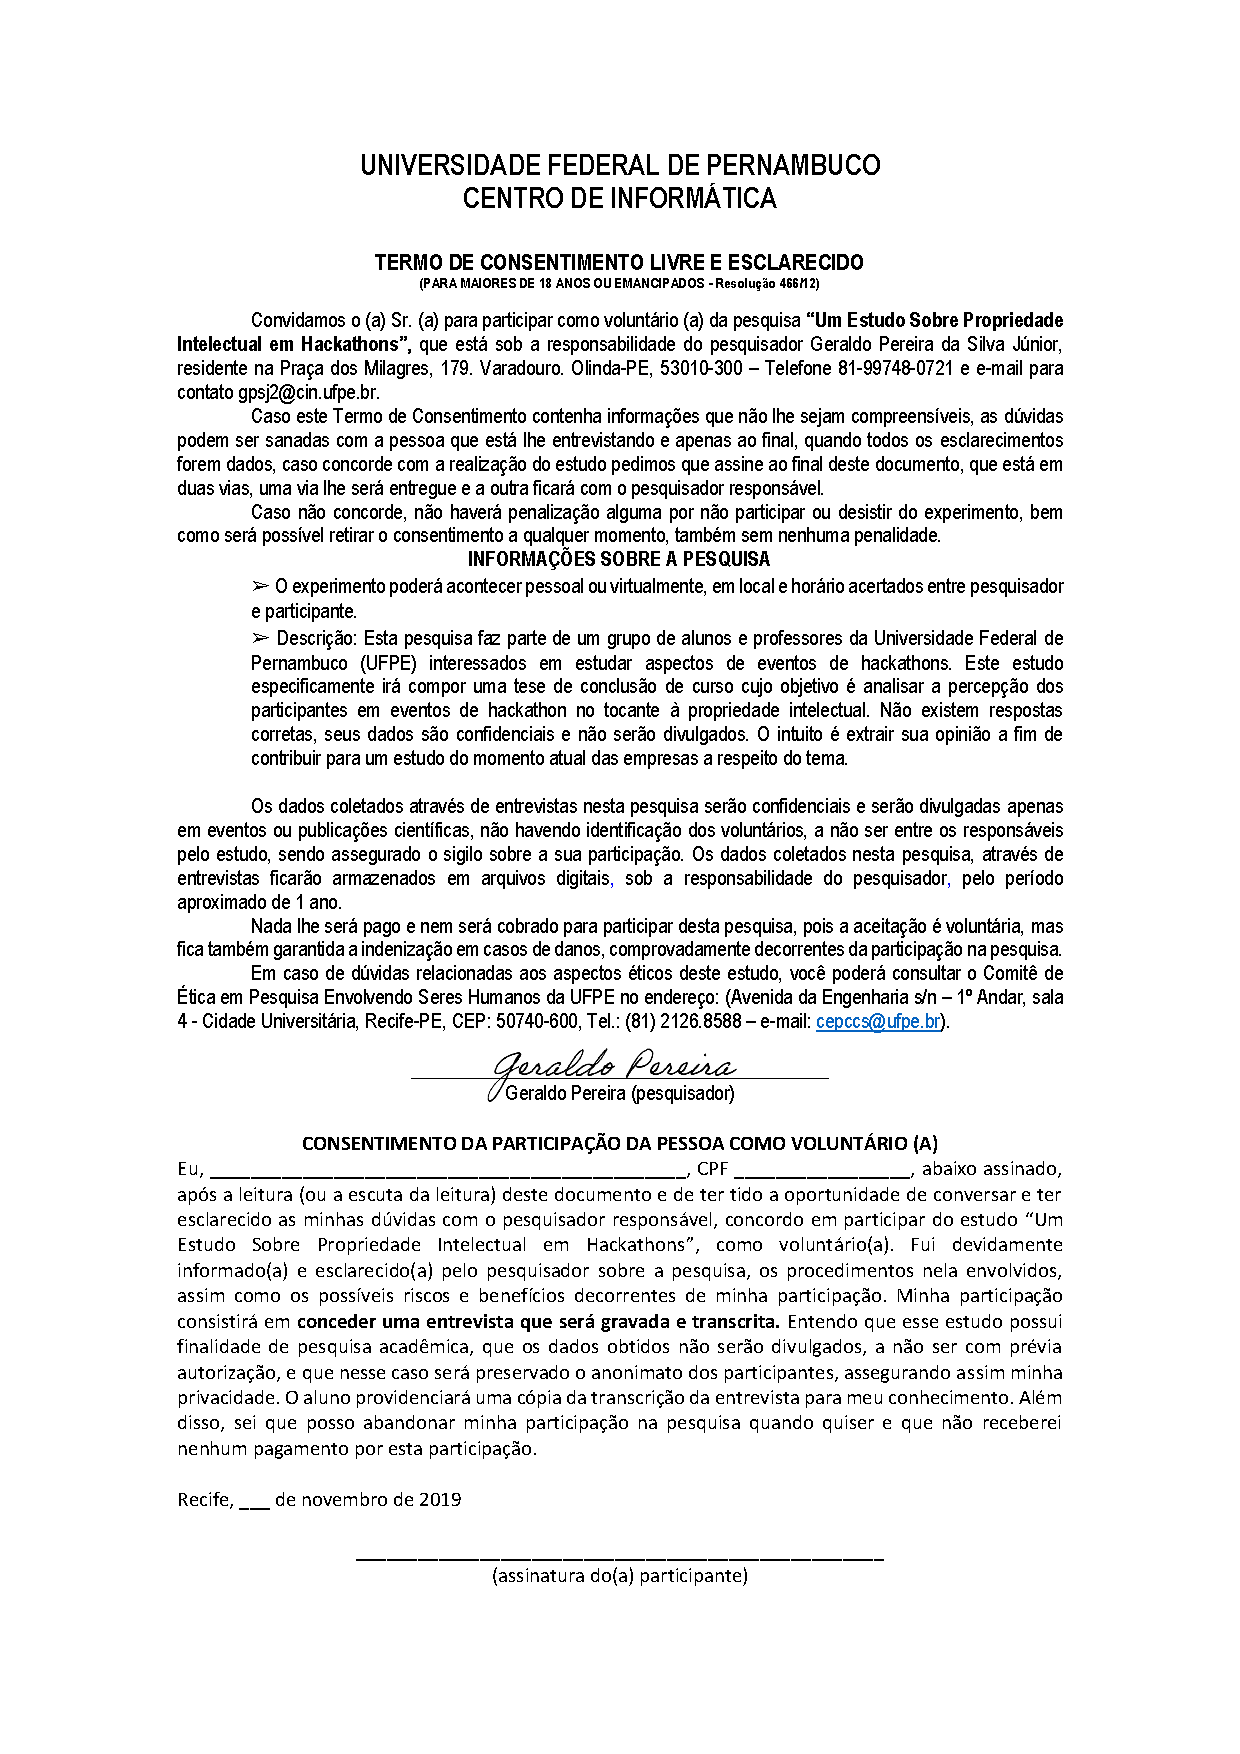
\includepdf[scale=0.80]{appendix/TermoConsentimento.pdf}
\end{minipage}
%%%%%%%%%%%%%%%%%%%%%%%%%%%%%%%%%%%%%%%%%%%%%%%%%%%%%%%%%%
%%%%%%%%%%%%%%%%%%%%%%%%%%%%%%%%%%%%%%%%%%%%%%%%%%%%%%%%%%

% APENDICE C

\chapter{Questionário}
\label{ap:questionario}
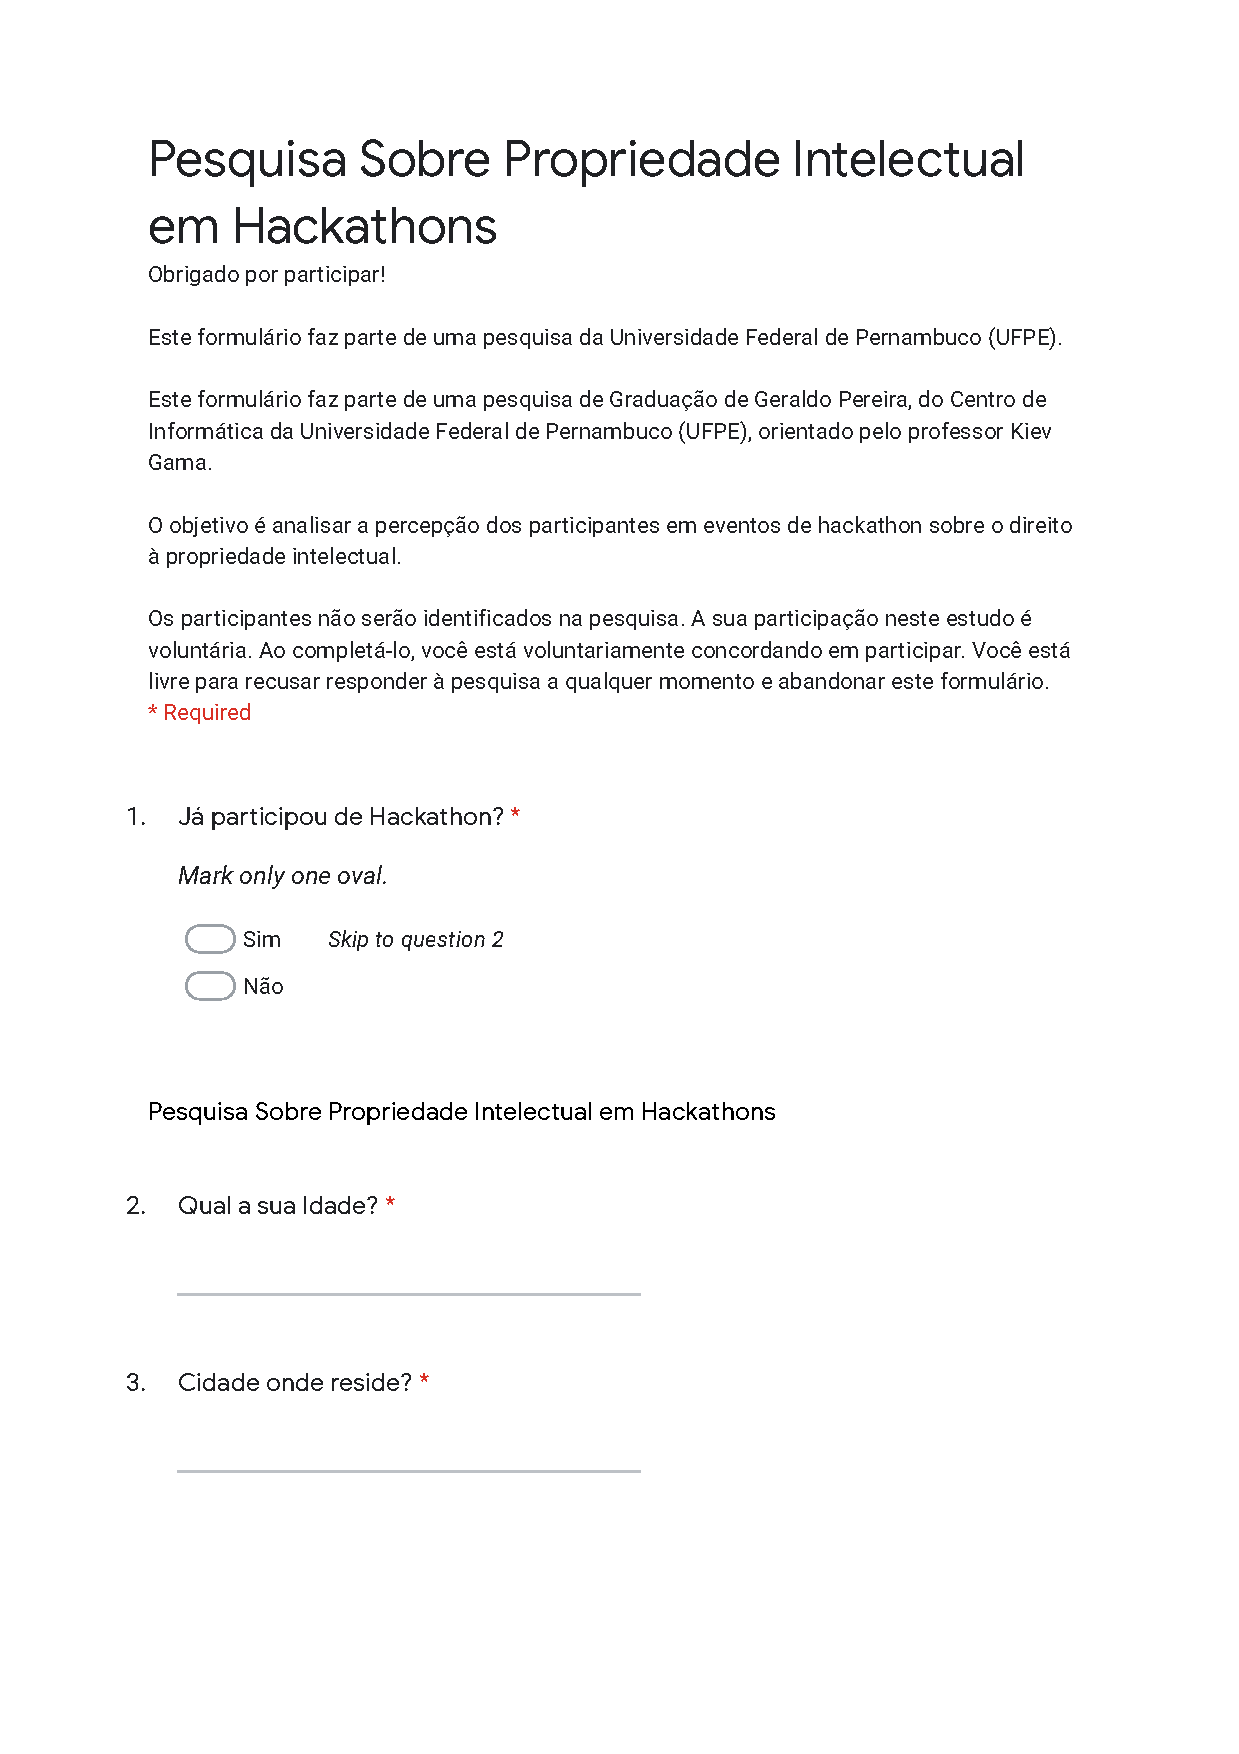
\includegraphics[scale=0.75]{appendix/FormularioGForm.pdf}

\includepdf[pages={2-6},width=\textwidth]{appendix/FormularioGForm.pdf}

%%%%%%%%%%%%%%%%%%%%%%%%%%%%%%%%%%%%%%%%%%%%%%%%%%%%%%%%%%
%%%%%%%%%%%%%%%%%%%%%%%%%%%%%%%%%%%%%%%%%%%%%%%%%%%%%%%%%%

% APENDICE D

\chapter{Nuvem de Palavras}
\label{ap:nuvem}

\begin{figure}[H]
    \centering
    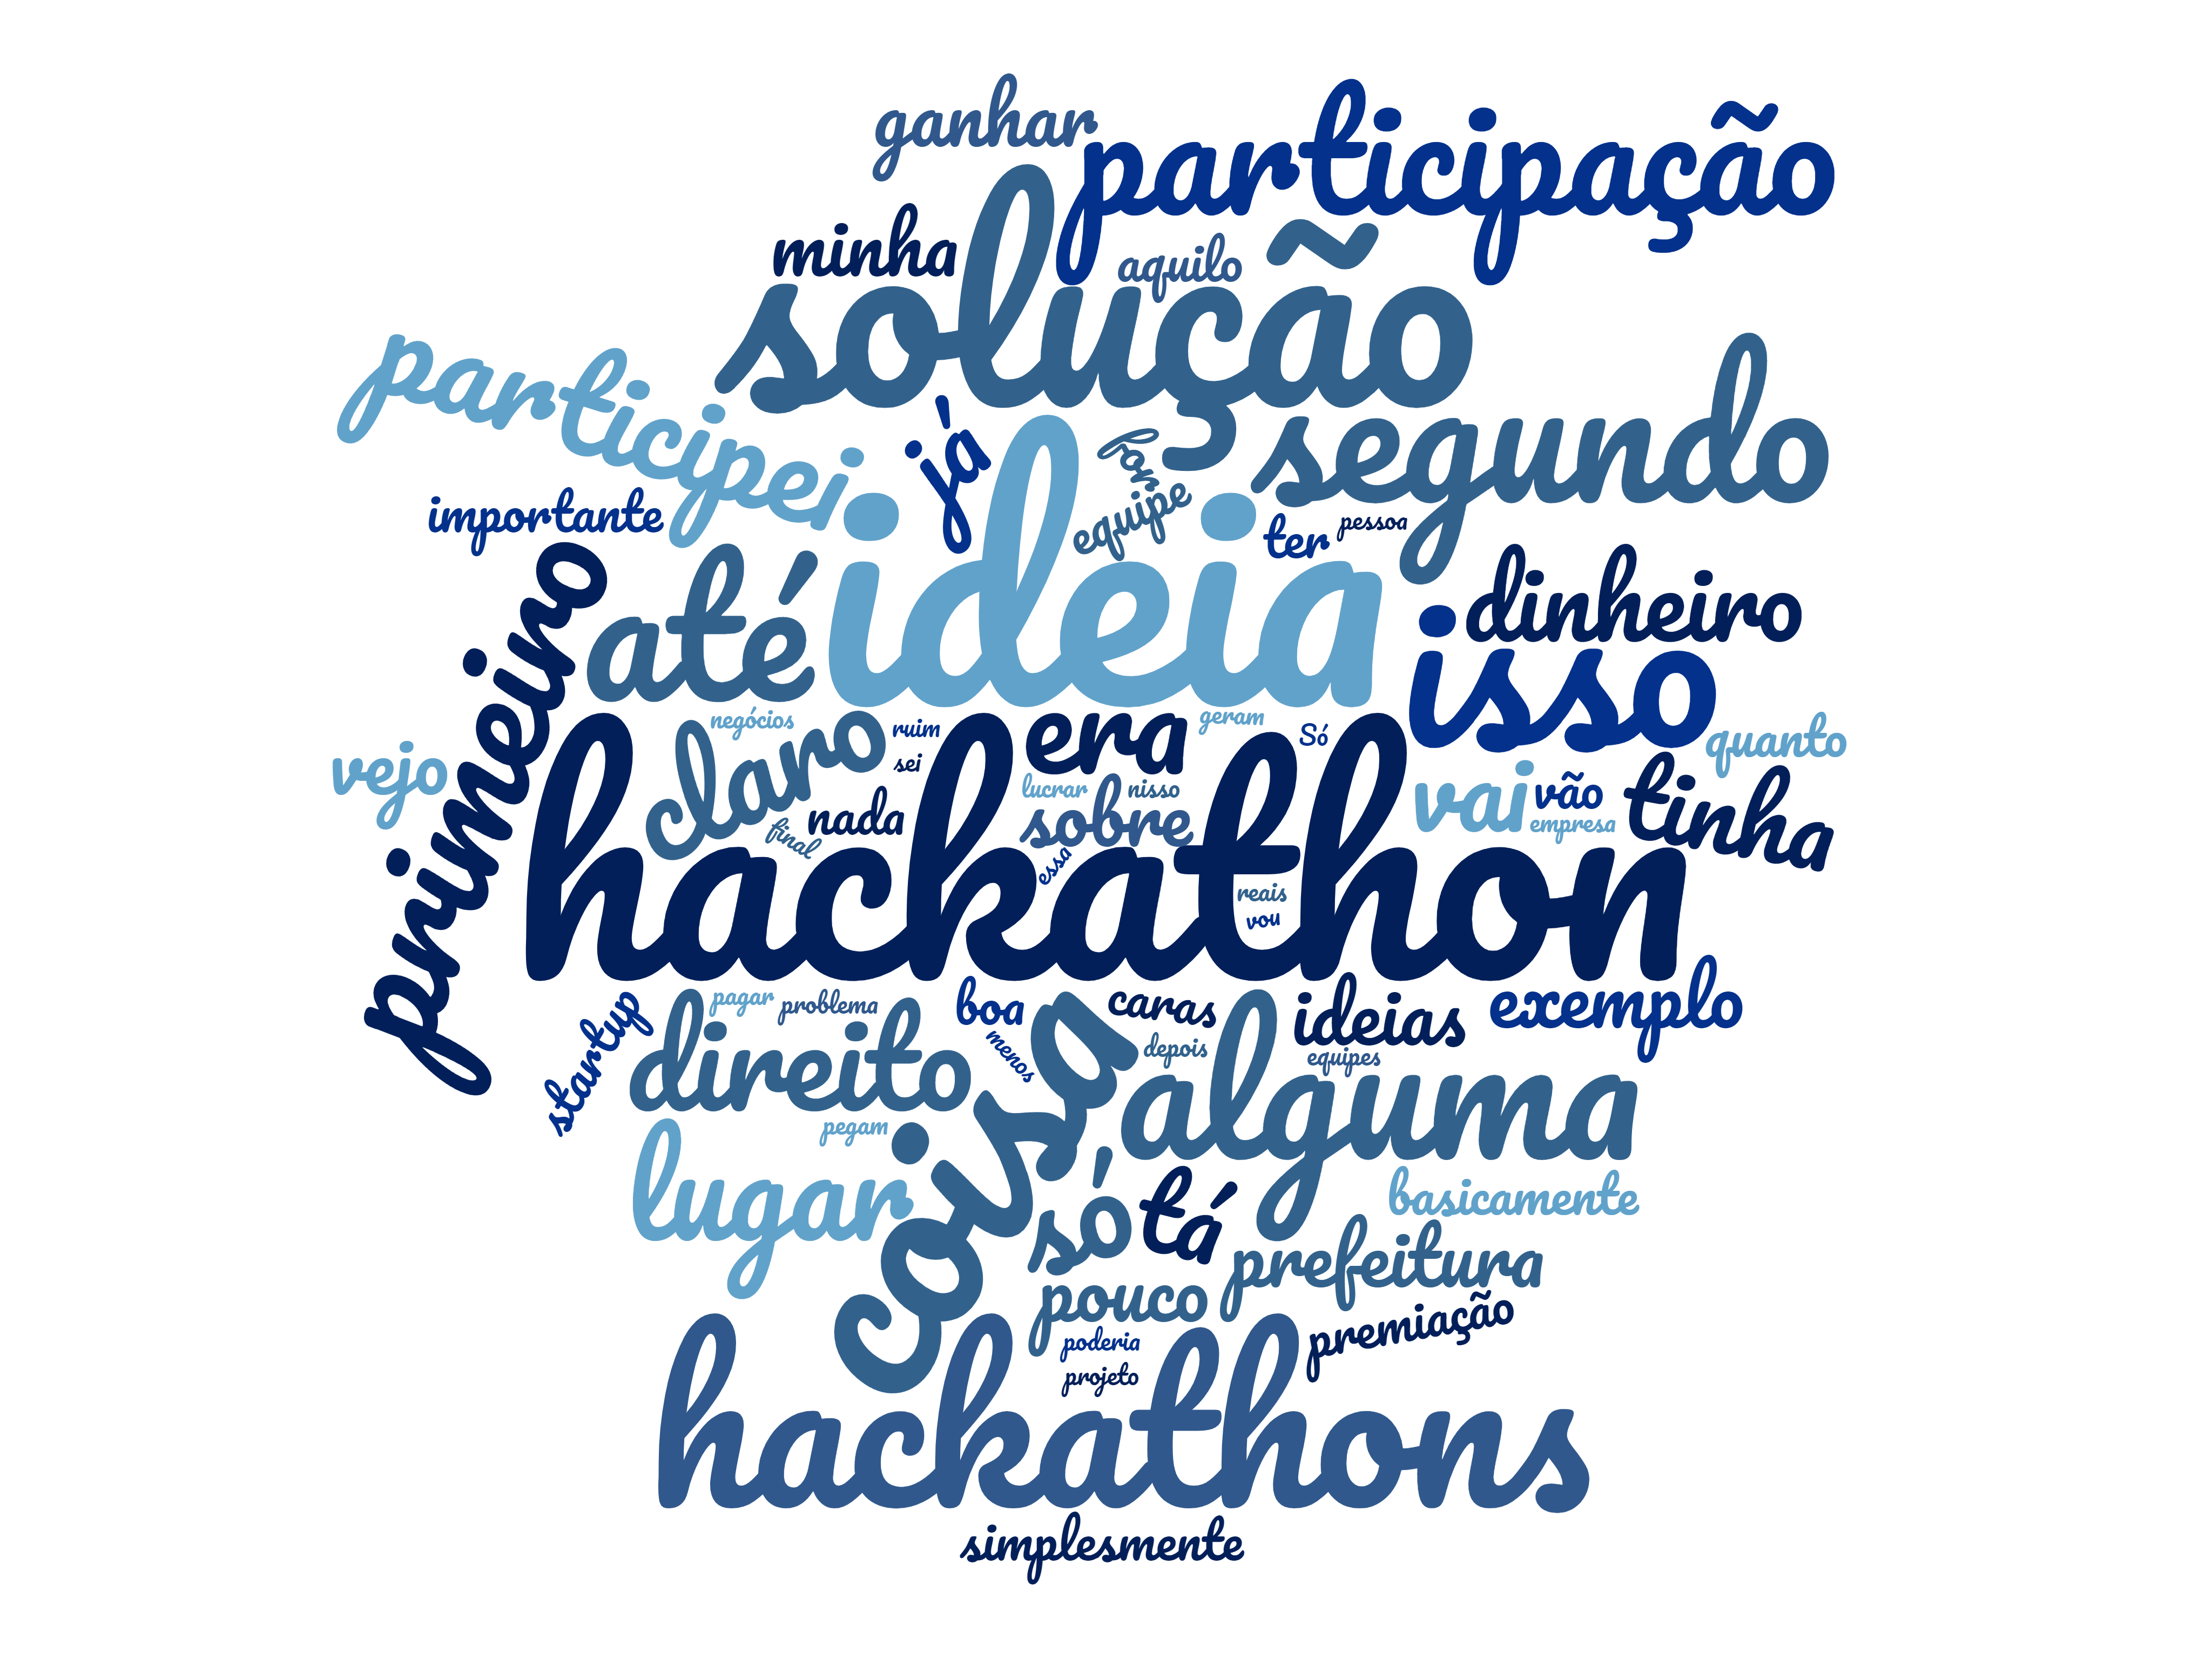
\includegraphics[width=0.7\textwidth]{appendix/wordcloud1.png}
    \caption{Nuvem de palavras do entrevistado 1}% nuvem 1
    \label{fig:nuvem-1}
\end{figure}

\begin{figure}[H]
    \centering
    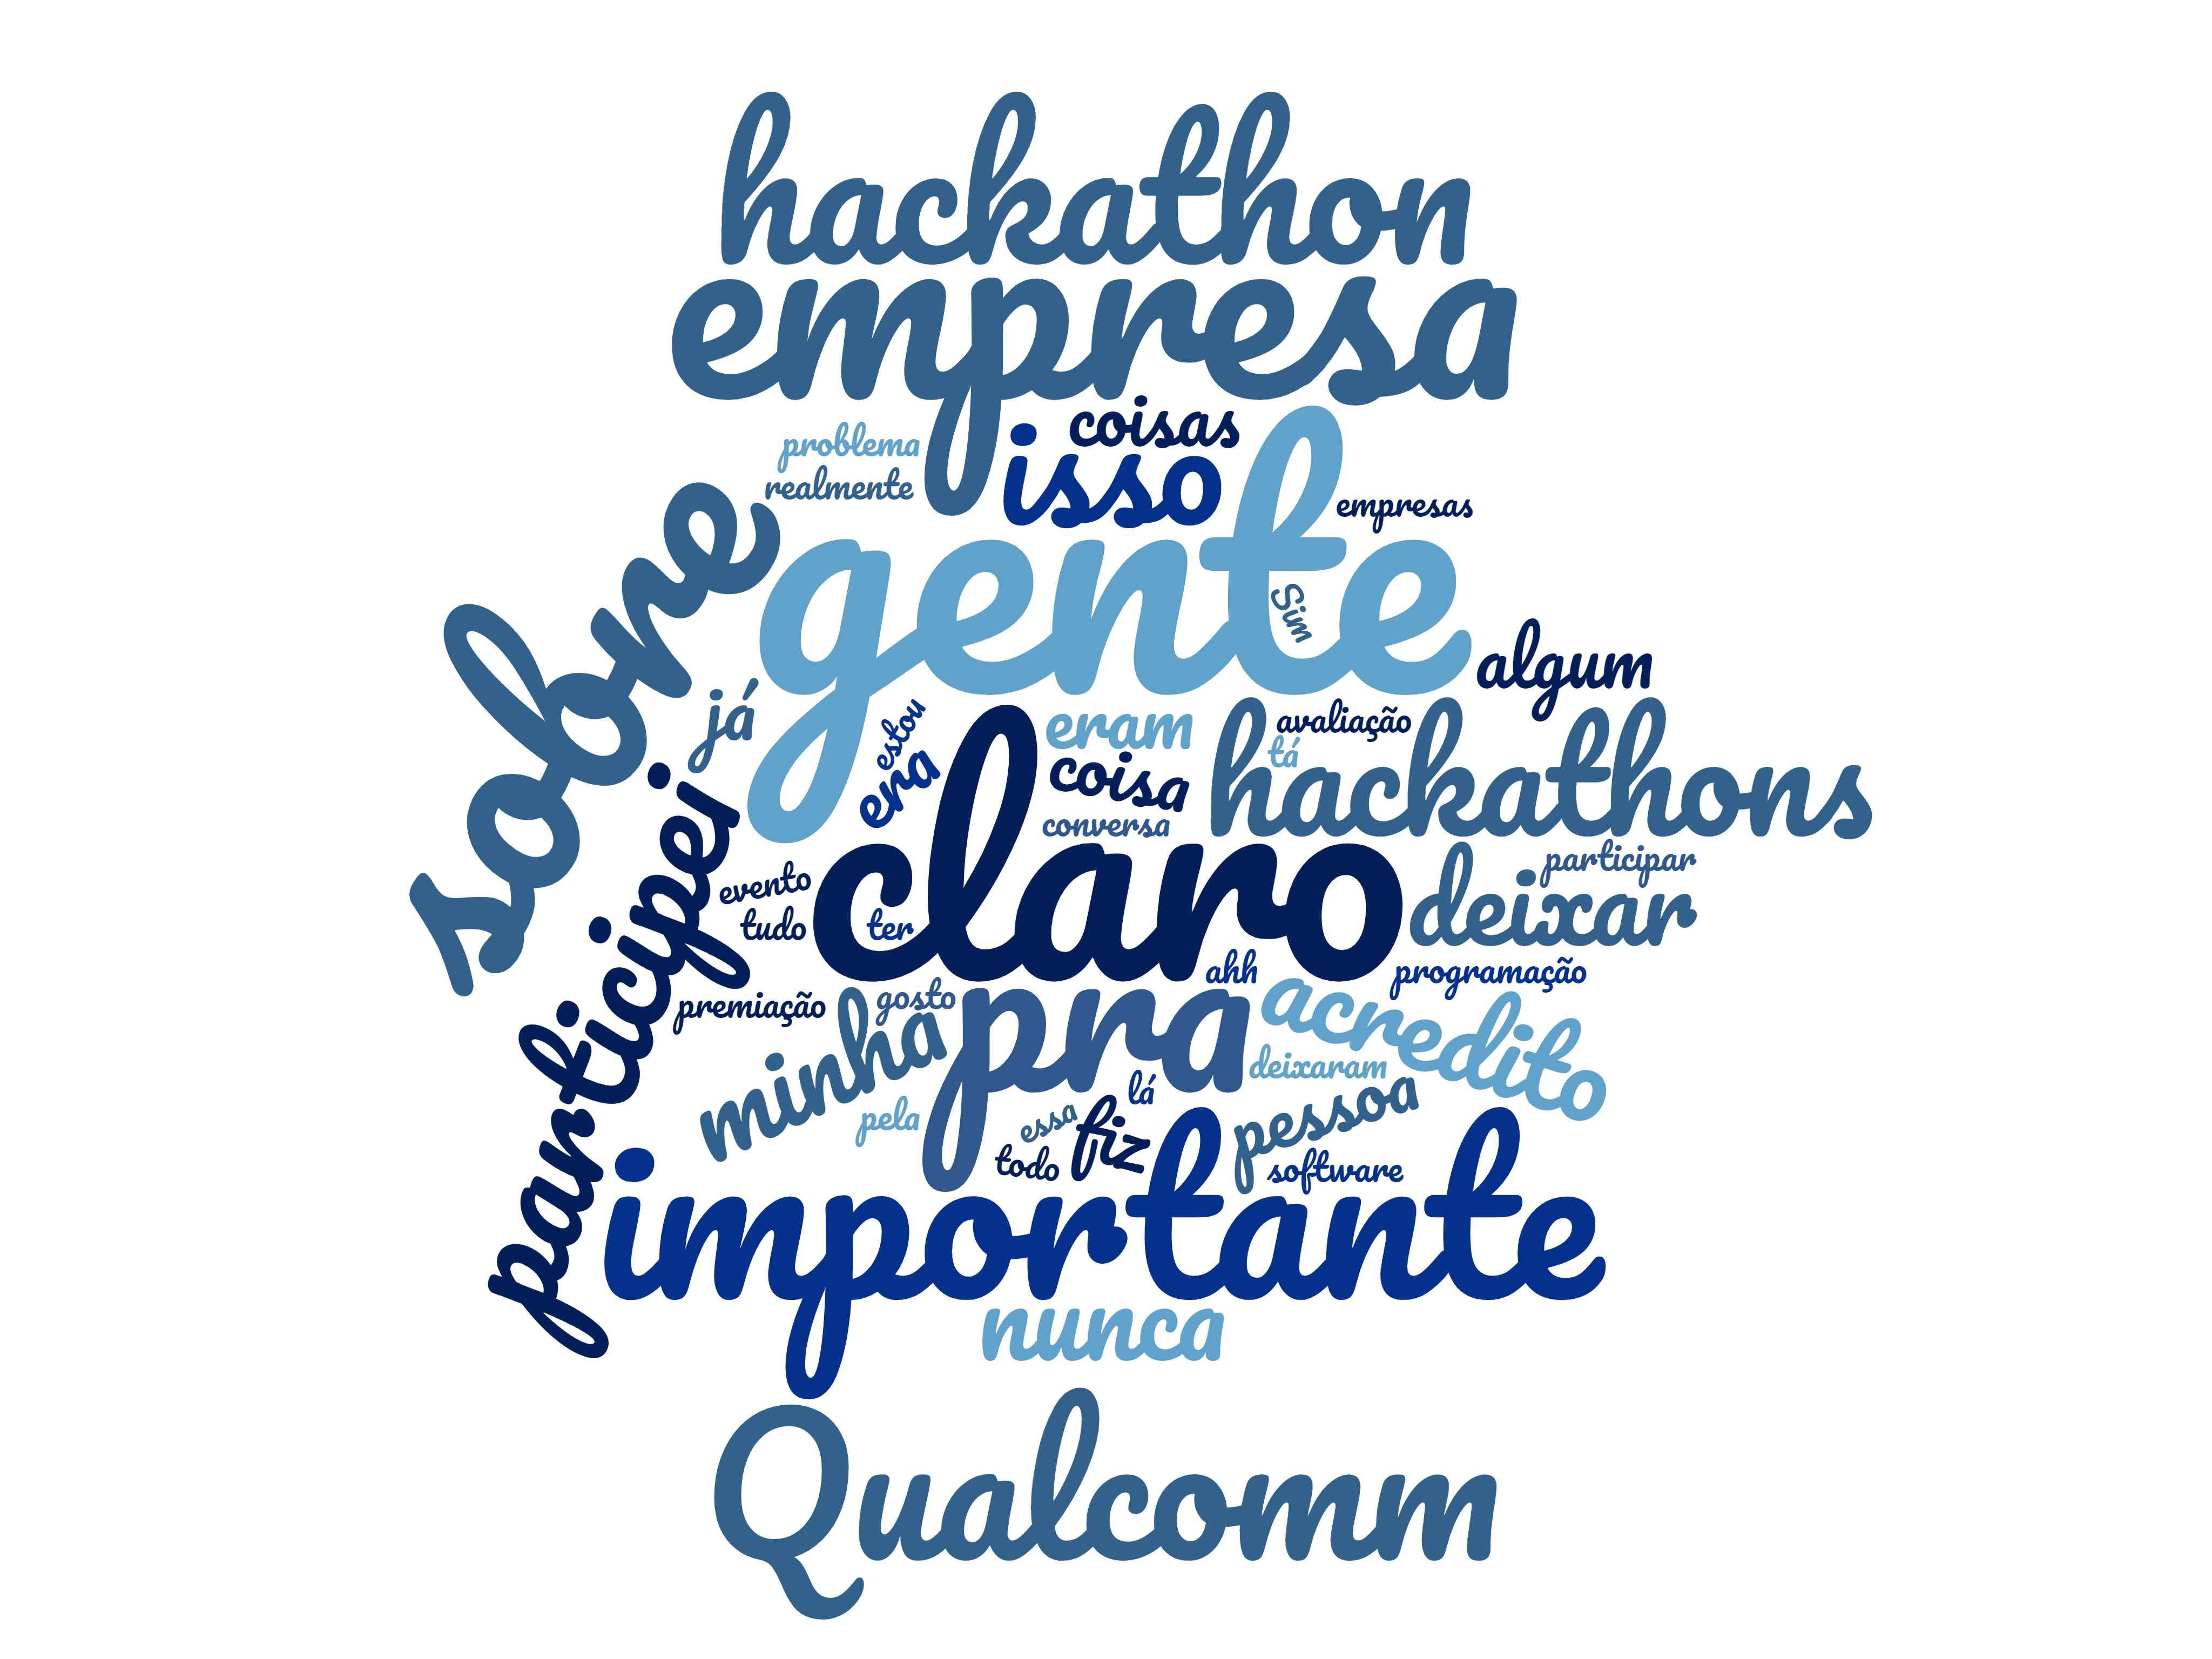
\includegraphics[width=0.7\textwidth]{appendix/wordcloud2.png}
    \caption{Nuvem de palavras do entrevistado 2}% nuvem 2
    \label{fig:nuvem-2}
\end{figure}

\begin{figure}[H]
    \centering
    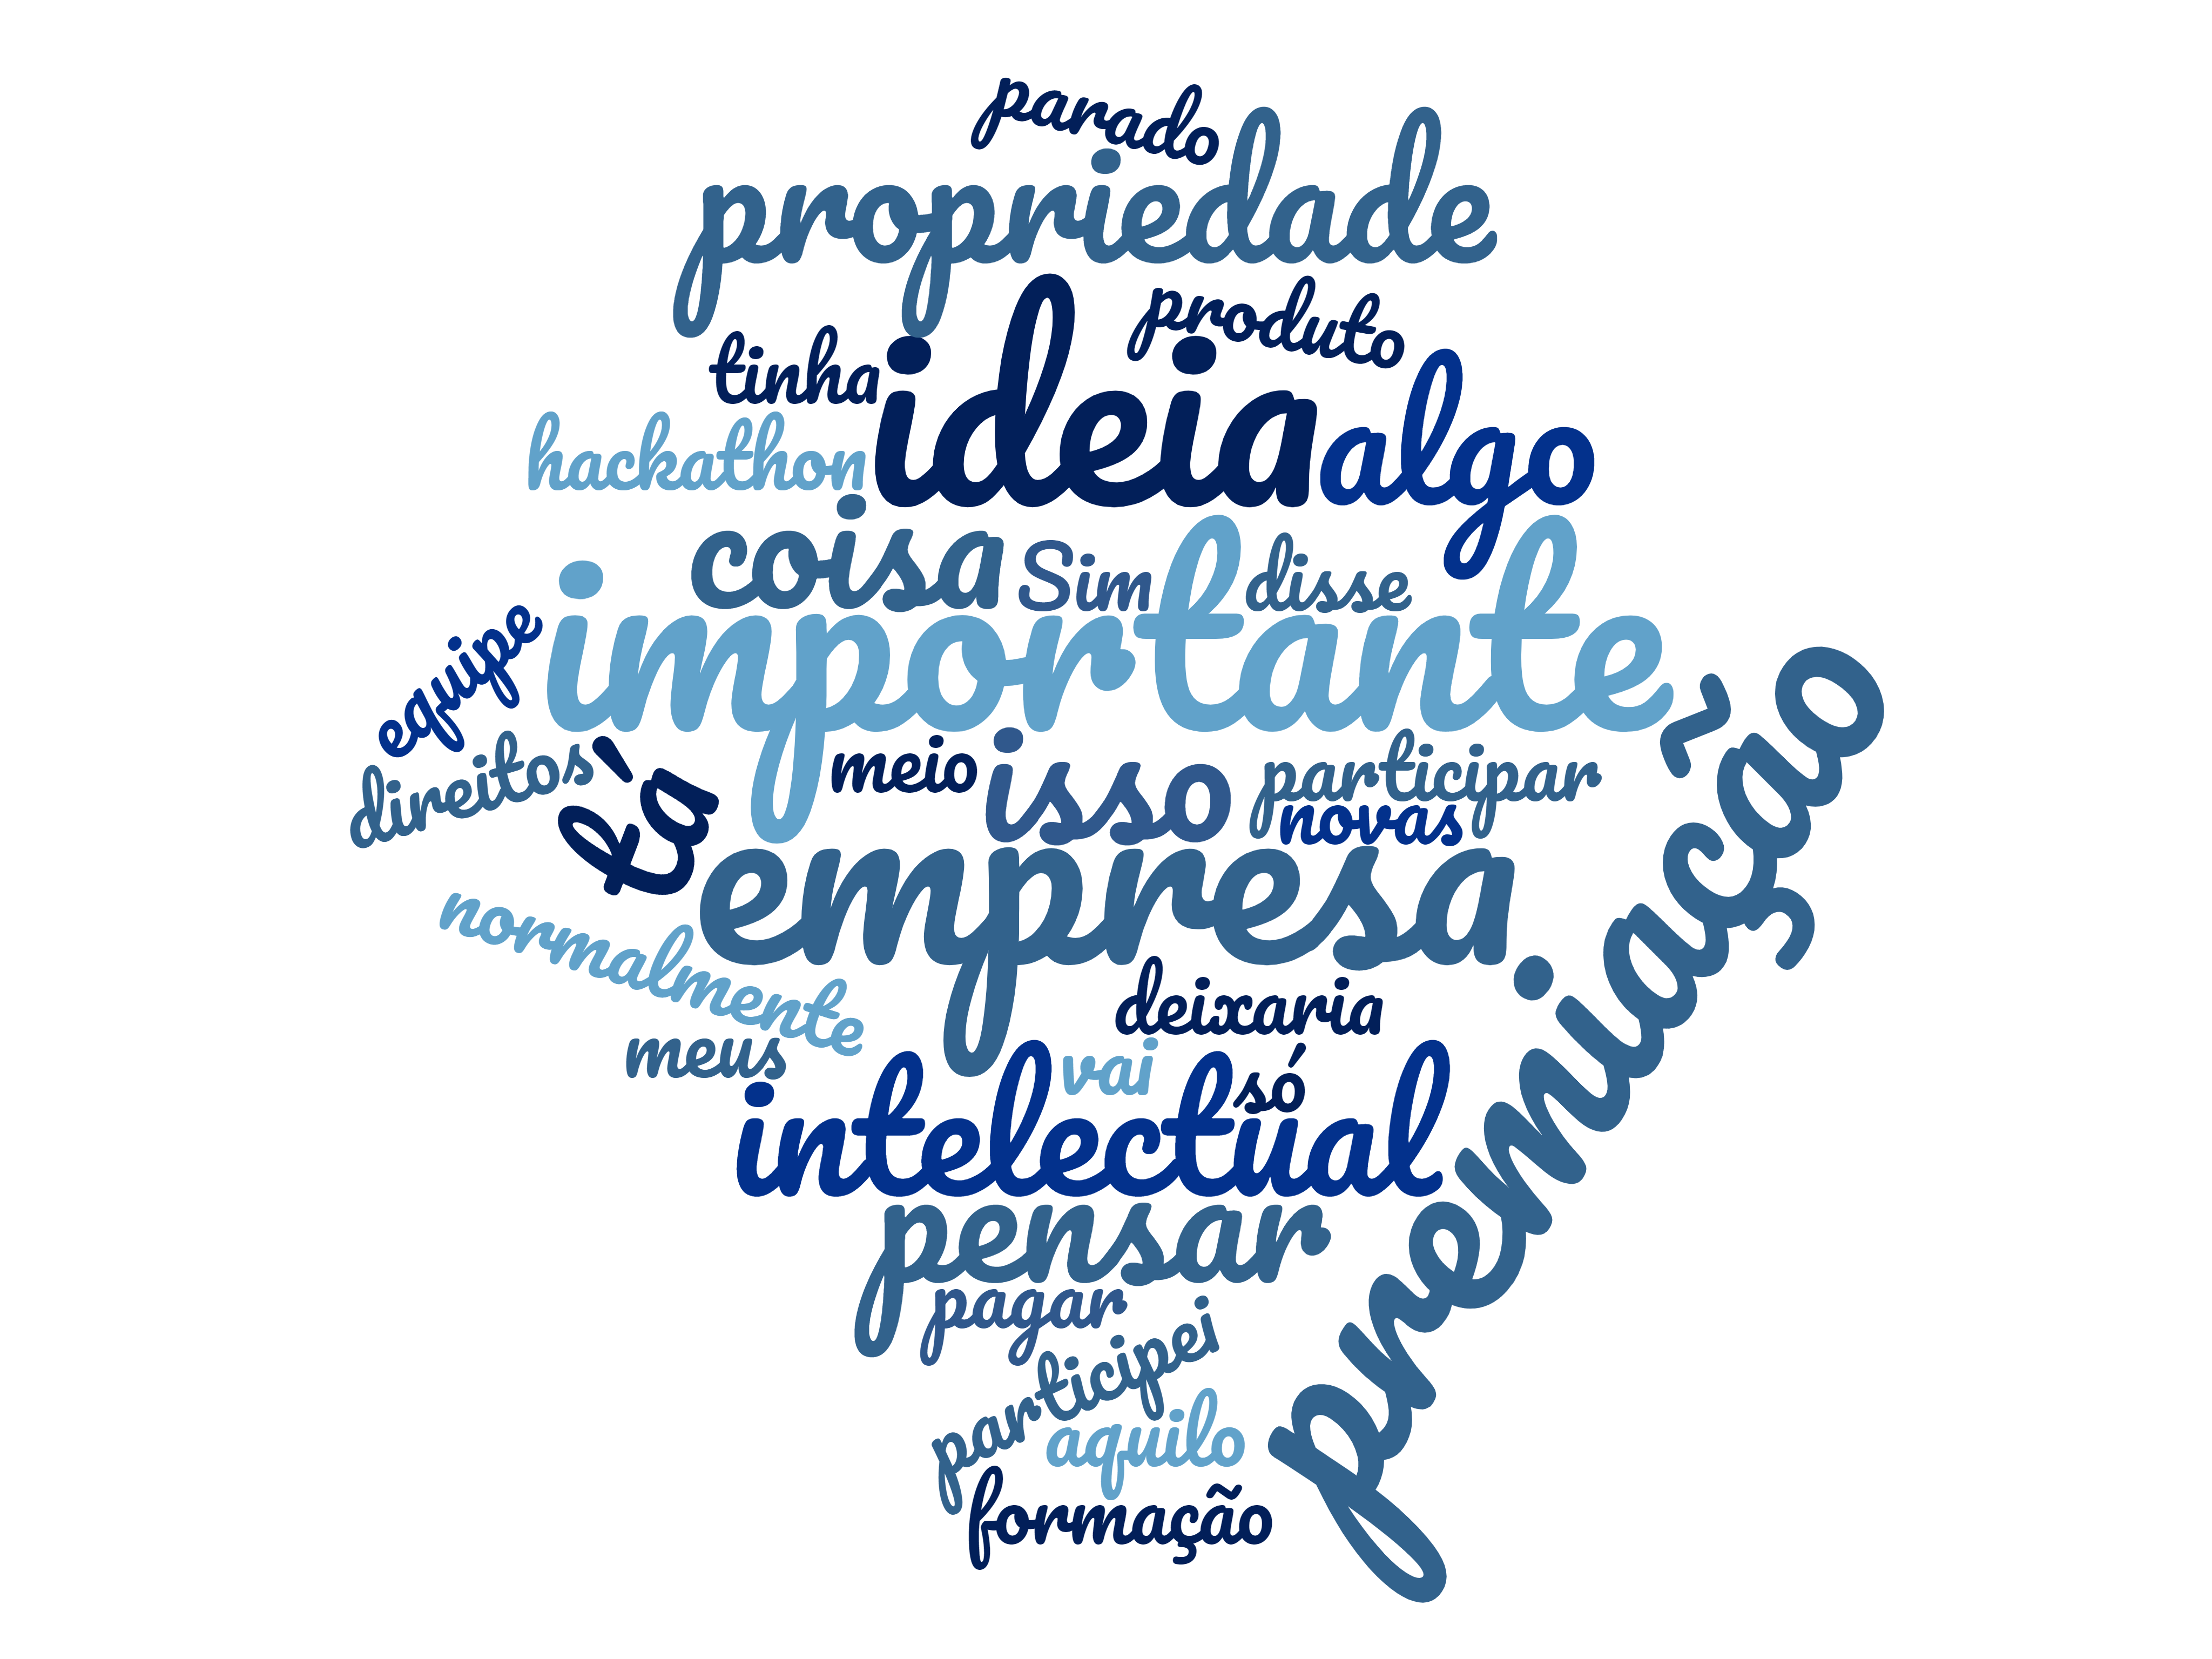
\includegraphics[width=0.7\textwidth]{appendix/wordcloud3.png}
    \caption{Nuvem de palavras do entrevistado 3}% nuvem 3
    \label{fig:nuvem-3}
\end{figure}

\begin{figure}[H]
    \centering
    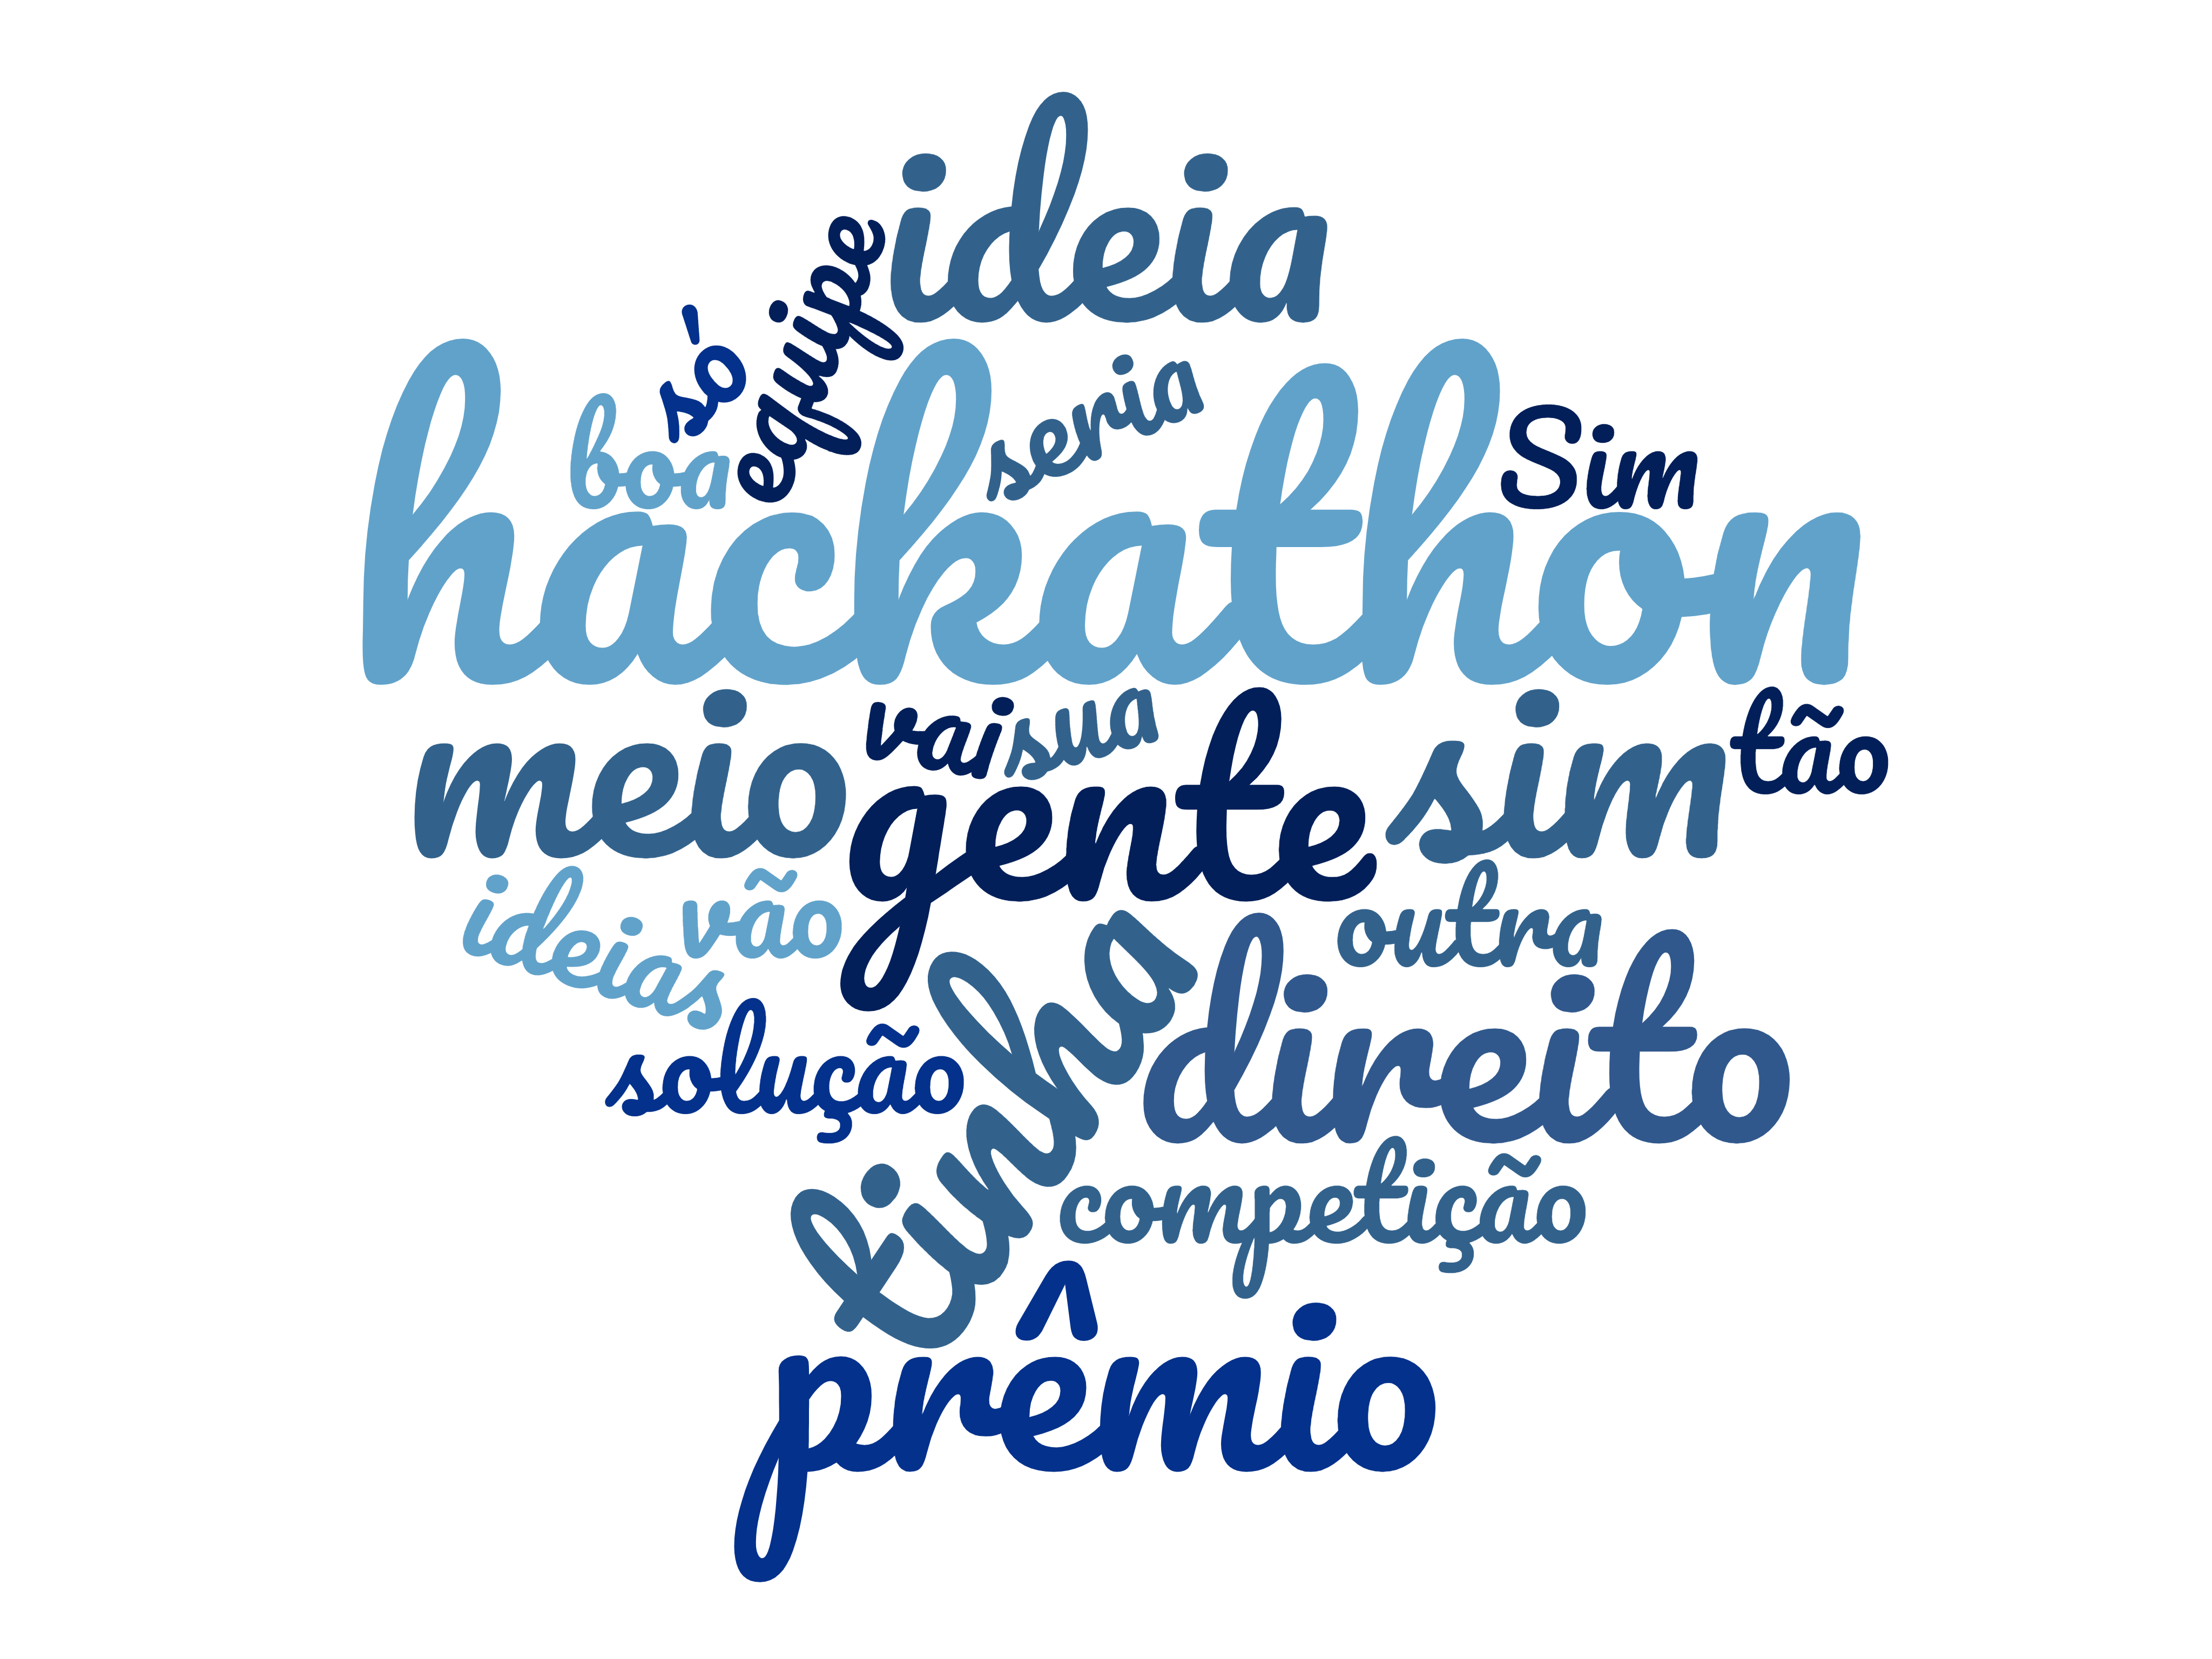
\includegraphics[width=0.7\textwidth]{appendix/wordcloud4.png}
    \caption{Nuvem de palavras do entrevistado 4}% nuvem 4
    \label{fig:nuvem-4}
\end{figure}

\begin{figure}[H]
    \centering
    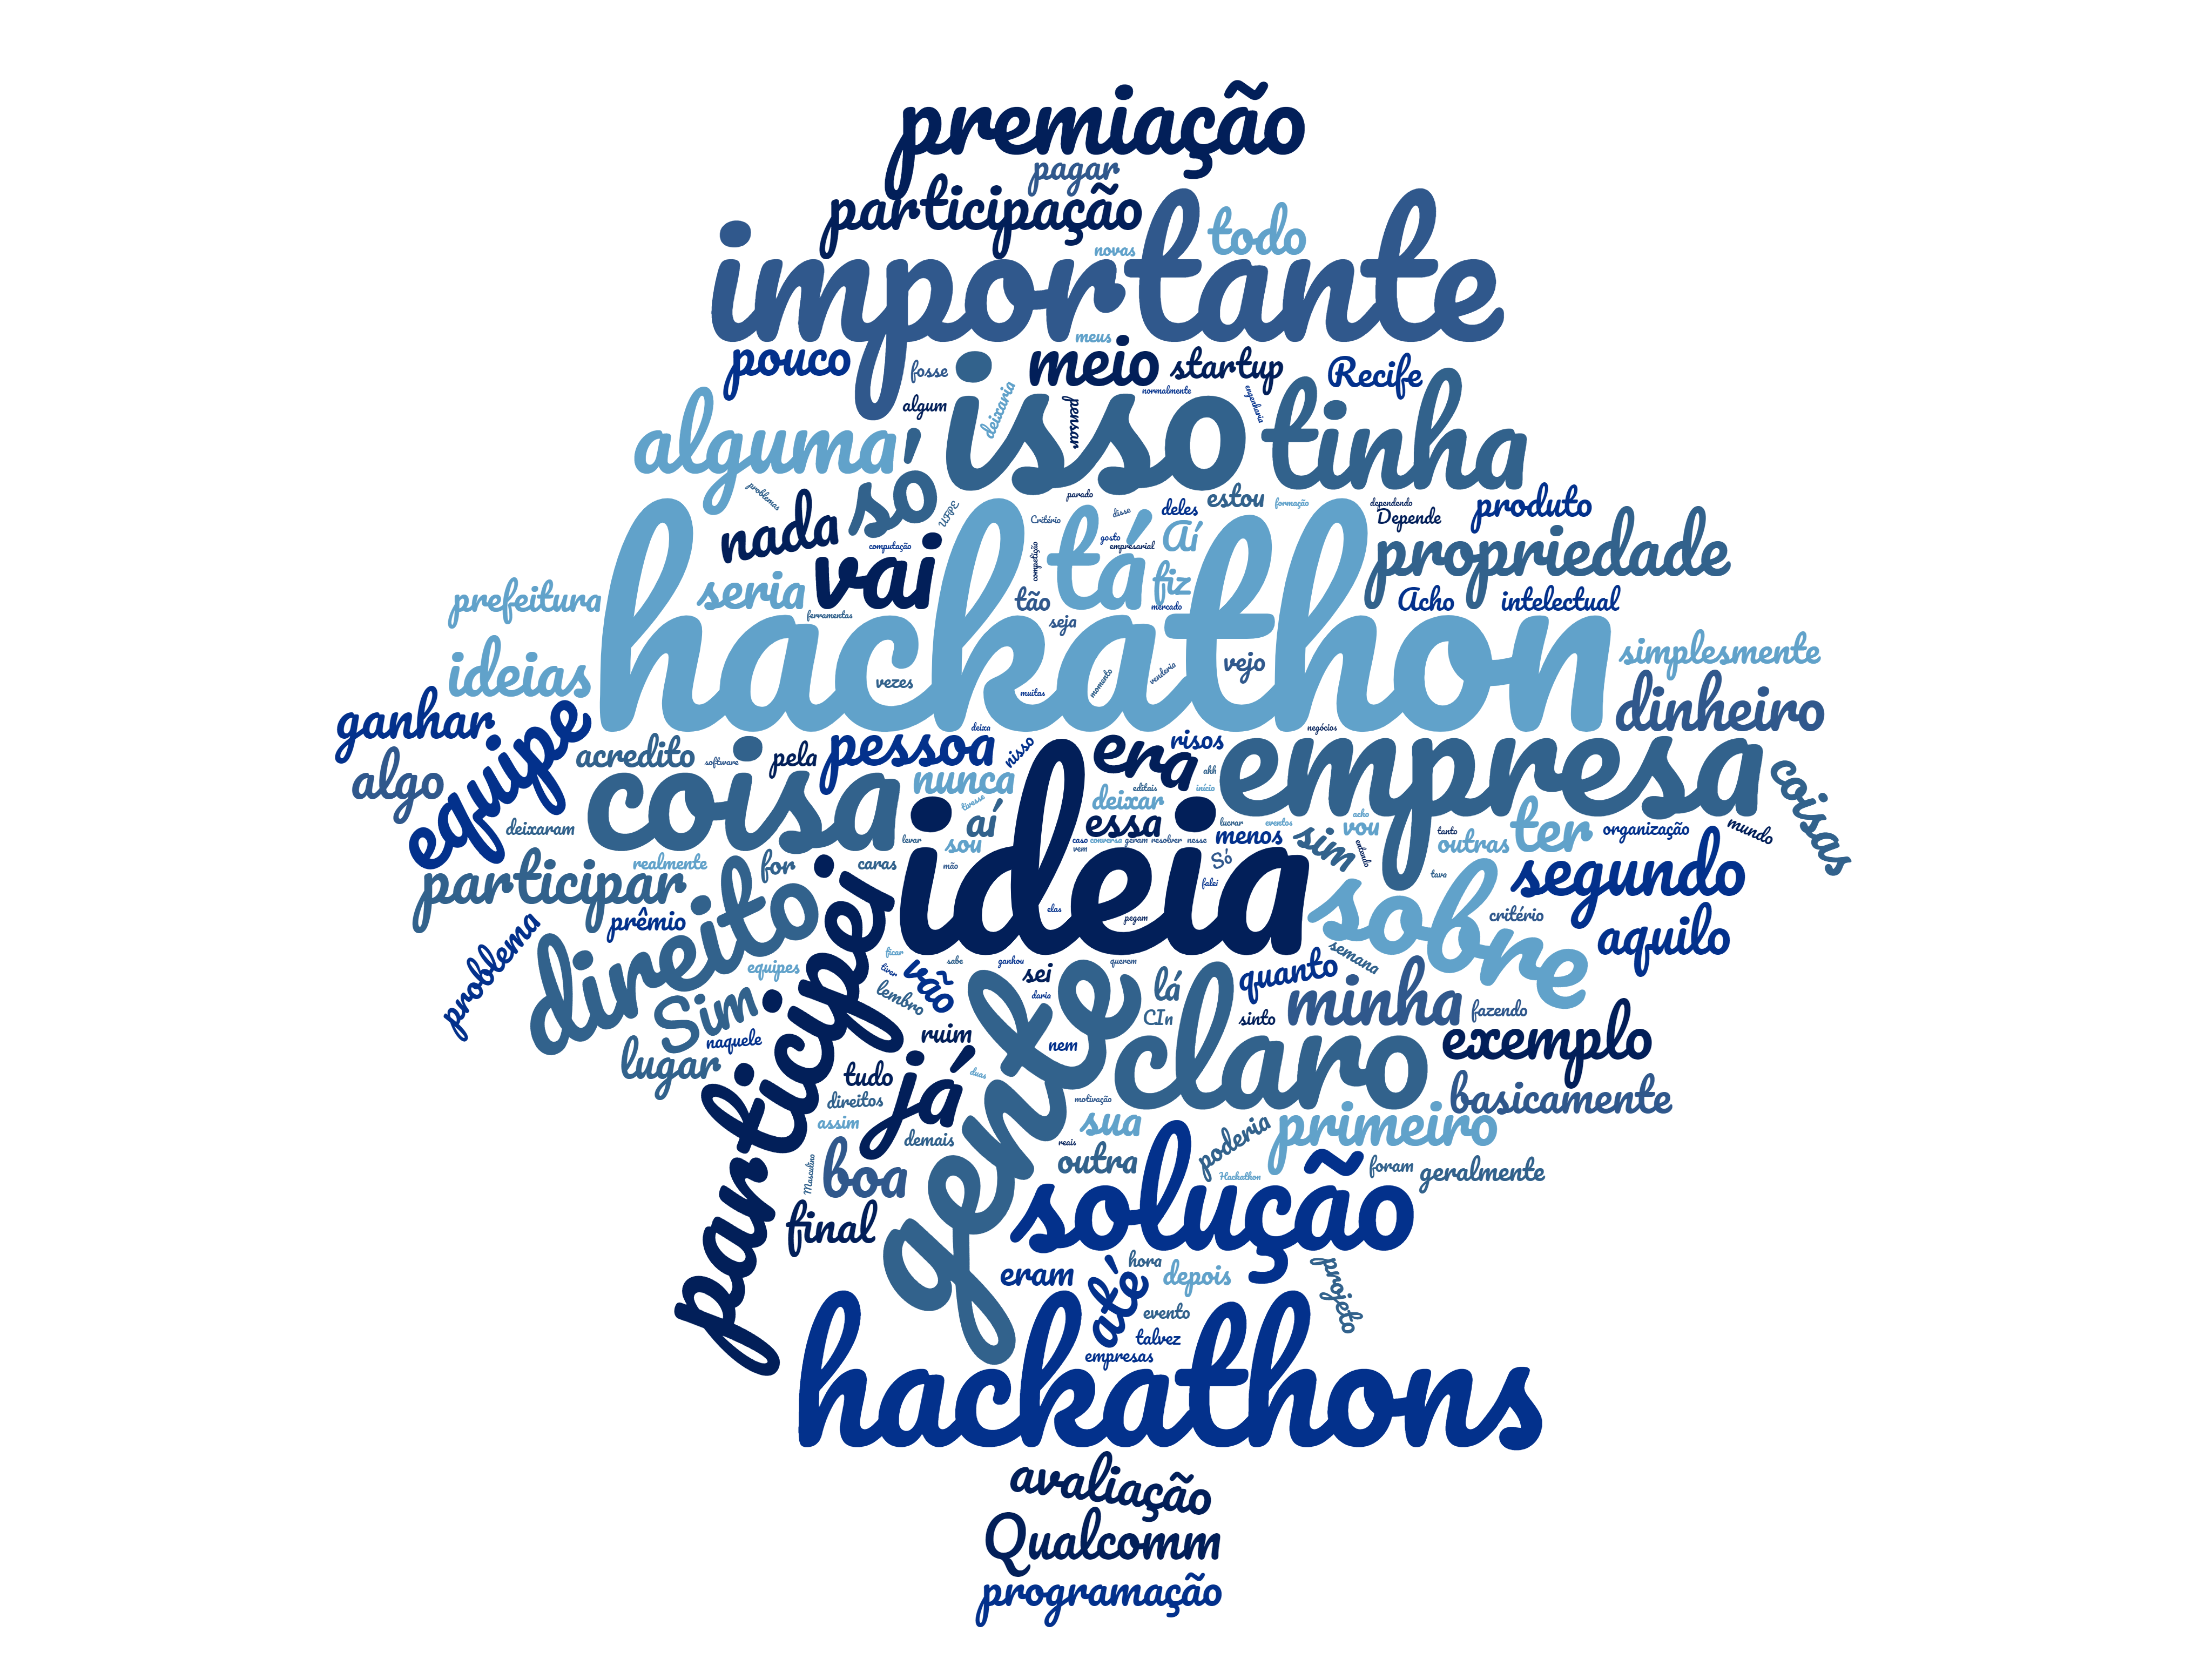
\includegraphics[width=1\textwidth]{appendix/wordcloudTODOS.png}
    \caption{Nuvem de palavras de todos os entrevistados}% nuvem geral
    \label{fig:nuvem-todos}
\end{figure}
\include{appendix/Termo}
\include{appendix/form}

\end{document}
